\begin{quoting}
Dans ce chapitre, vous apprendrez comment faire
du pain au levain de blé autonome.
\end{quoting}

\begin{figure}[!htb]
  \includegraphics[width=\textwidth]{loaf-pan-free-standing.jpg}
  \caption[Pain autonome et pain en moule]{Un pain au levain autonome
      à côté d'un pain fait dans un moule.  Le levain autonome est considéré
      comme la discipline suprême du pain au levain par de nombreux boulangers.}
\end{figure}

Le pain au levain autonome est mon type de pain préféré. Il allie une superbe croûte croustillante, une saveur supérieure et une mie moelleuse et légère. C'est le type de pain qui est consommé à toute vitesse par mes amis et ma famille. Malheureusement, faire ce type de pain demande beaucoup plus d'efforts, de patience et de technique que les autres types de pain. Vous devez parfaitement équilibrer le processus de fermentation. Vous ne pouvez pas fermenter trop peu ou trop longtemps. Les techniques que vous devez apprendre nécessitent un peu plus de compétences. Il m'a fallu plusieurs tentatives pour réussir. L'un des défis auxquels j'ai été confronté était que j’avais la mauvaise farine. Je ne savais pas correctement utiliser mon four. Quand devrais-je arrêter la fermentation ? Il y a beaucoup d'informations disponibles. J'ai passé au crible la plupart d'entre elles et j'ai tout essayé. Dans de nombreux cas, les informations étaient incorrectes; dans d'autres cas, j’ai trouvé une autre pièce de puzzle précieuse. Rassembler toutes ces informations a été l'une de mes principales motivations pour commencer Le Code du Pain. Mon principal apprentissage a été qu'il n'y a pas de recette que vous pouvez suivre aveuglément. Vous devrez toujours adapter la recette à vos outils et à votre environnement locaux.

Mais ne vous inquiétez pas. Après avoir lu ce chapitre, vous saurez tous les signes à repérer. Vous serez en mesure de lire votre pâte. Vous deviendrez un boulanger amateur confiant qui peut faire du pain à la maison, en haute altitude, en basse altitude, en été, en hiver, chez vos amis, et même en vacances. De plus, vous saurez comment augmenter votre production de 1 à 100 pains. Si vous avez déjà voulu ouvrir une boulangerie, considérez ces connaissances comme votre base.

Maîtriser ce processus vous permettra de faire du pain incroyable qui a beaucoup meilleur goût que n'importe quel pain acheté en magasin.

\section{Le processus}

\begin{flowchart}[!htb]
\begin{center}
  \begin{tikzpicture}[node distance = 3.2cm, auto]
  \node [start] (init) {Ready starter};
  \node [block, right of=init] (mix_ingredients) {Mix ingredients};
  \node [block, right of=mix_ingredients] (dough_strength) {Create dough strength};
  \node [block, right of=dough_strength] (bulk) {Bulk ferment};
  \node [decision, below of=bulk] (divide_test) {Making one loaf?};
  \node [block, right of=divide_test] (divide) {Divide};
  \node [block, below of=divide] (preshape) {Preshape};
  \node [block, below of=divide_test] (shape) {Shape};
  \node [block, left of=shape] (proof) {Proof};
  \node [success, left of=proof] (bake) {Bake};
  \path [line] (init) -- (mix_ingredients);
  \path [line] (mix_ingredients) -- (dough_strength);
  \path [line] (dough_strength) -- (bulk);
  \path [line] (bulk) -- (divide_test);
  \path [line] (divide_test) -- node{yes} (shape);
  \path [line] (divide_test) -- node{no} (divide);
  \path [line] (divide) -- (preshape);
  \path [line] (preshape) -- (shape);
  \path [line] (shape) -- (proof);
  \path [line] (proof) -- (bake);
\end{tikzpicture}

  \caption{Le processus typique de fabrication d'un pain au levain à base de blé.}%
  \label{fig:wheat-sourdough-process}
\end{center}
\end{flowchart}

Tout le processus de fabrication d'un excellent pain au levain commence par la préparation de votre levain. La clé pour maîtriser ce processus est de gérer correctement le processus de fermentation. Pour cela, la base est d'avoir un levain actif et sain.

Une fois que votre levain est prêt, vous passez au mélange de tous les ingrédients. Vous voulez homogénéiser correctement votre levain. De cette façon, vous assurez une fermentation uniforme sur toute votre pâte.

Après une courte pause, vous allez procéder à la création de la force de la pâte. Le pétrissage va créer un réseau de gluten fort. Cela est essentiel pour piéger correctement le \ch{CO2} produit pendant la fermentation.

Une fois que vous avez pétri, la fermentation en masse commence. On l'appelle fermentation en masse parce que vous faites généralement fermenter plusieurs pains ensemble en un seul lot. Comprendre quand arrêter cette étape demandera un peu de pratique. Mais ne vous inquiétez pas, vous apprendrez à reconnaître exactement les signes à surveiller.

Une fois cela terminé, vous devez diviser votre gros bloc de pâte en morceaux plus petits et pré-former chaque pièce. Cela vous permet d'appliquer plus de force à la pâte et de créer des pains de forme plus uniforme.

L'étape de l'épreuve suit, où vous terminez le processus de fermentation. Selon votre temps, vous pouvez faire l'épreuve à température ambiante ou au frigo. Maîtriser l'épreuve transformera votre bon pain en un excellent pain.Enfin, vous terminerez tout le processus par la cuisson. Vous apprendrez différentes
options sur comment bien cuire votre pâte. De cette façon, votre
pâte aura une belle levée au four. Pendant la deuxième
étape du processus de cuisson, vous finirez de construire votre croûte.

Toutes les étapes dépendent les unes des autres. Il vous faudra réussir chacune
des étapes pour faire le pain parfait.

\section{Préparation de votre levain}%
\label{section:préparation-levain}

La partie la plus cruciale du processus de fabrication du pain est votre levain.
Le levain est ce qui commence la fermentation dans votre pâte principale.
Si votre levain est défectueux, alors votre pâte principale va également 
causer des problèmes pendant la fermentation. Les propriétés de votre levain
sont transmises à votre pâte principale. Si votre levain
n'a pas un bon équilibre de levure à bactéries, votre
pâte principale le sera aussi.

En général, considérez la pâte que vous mélangez comme un gros levain avec du sel.
Après avoir mélangé tous les ingrédients, vous avez à nouveau un environnement vierge.
La levure et les bactéries recommencent à se battre pour prendre le dessus les unes sur les autres.
Il y a beaucoup de nourriture disponible, et elles font toutes de leur mieux pour gagner.
En fonction du levain que vous mélangez dans votre pâte, certains des micro-organismes
pourraient avoir un avantage sur les autres.

La première option pour obtenir un bon équilibre est d'appliquer des nourrissages.
Si votre levain n'a pas été nourri pendant une longue période, les
bactéries dominent. Cela se produit si votre levain a été
assis inutilisé dans le réfrigérateur, par exemple. À mesure que de plus en plus
d'acidité s'accumule, l'environnement devient de plus en plus hostile
à la levure. Les bactéries lactiques tolèrent cet environnement
mieux. La fermentation de votre pâte serait plus du côté
bactérien avec ce levain. En appliquant quelques
nourrissages, la levure devient plus active. Plus votre
levain est vieux, plus la levure devient résistante aux acides. Au début,
j'ai dû nourrir mon levain 2-3 fois pour rééquilibrer le balance. Avec mon
levain plus mature, un nourrissage semble suffire pour équilibrer
les micro-organismes.

Certaines personnes utilisent un ratio 1:1:1 pour rafraîchir le levain. Ce serait
une partie de l'ancien levain (\qty{10}{\gram} par exemple), 1 partie de farine,
et une partie d'eau. Je pense que c'est du grand n'importe quoi. Comme mentionné
votre levain est une énorme pâte. Vous n'opteriez jamais pour un ratio 1:1:1 pour
faire de la pâte. Vous pourriez utiliser un maximum de \qty{20}{\percent} de levain pour
faire de la pâte. C'est pourquoi je préconise d'utiliser un ratio 1:5:5 ou un
ratio 1:10:10 selon la maturité de votre levain. Comme j'utilise presque
toujours un levain plus raide en raison de ses avantages pour la fermentation de la levure
(voir Section~\ref{section:levain-raide})
mon ratio n'est jamais 1:5:5. Mon ratio serait 1:5:2.5 (1 partie d'ancien levain,
5 parties de farine, 2.5 parties d'eau). Si il fait très chaud là où vous vivez
vous pourriez opter pour le 1:10:5 ou 1:20:10 mentionné précédemment. De cette
façon, vous ralentissez la maturation de votre levain. Vous pouvez également utiliser cette
astuce pour faire coïncider l'alimentation de votre levain avec votre emploi du temps.
Si votre levain est généralement prêt en 6 heures mais qu'aujourd'hui, vous en avez besoin
plus tard, augmentez simplement la quantité de farine/eau que vous donnez à votre levain.
Ce sont toutes des valeurs que vous devez expérimenter par vous-même.
Chaque levain est unique et peut se comporter légèrement différemment.La deuxième option à votre disposition est la quantité de levain que vous utilisez pour faire la pâte. Comme indiqué précédemment, votre levain se régénère dans votre pâte principale. Bien que je~normalement utiliser entre \qtyrange{10}{20}{\percent} de levain sur la base de la farine, parfois je~descends à \qty{1}{\percent} de levain. De cette façon, les micro-organismes ont plus de place pour se rééquilibrer lors de la fermentation de la pâte. Si mon levain n'a pas été nourri pendant une journée, je~pourrais utiliser \qty{5}{\percent} de levain pour faire une pâte. Si je~pousse cela à 2 jours sans nourriture, je~réduis encore plus la quantité de levain. Je~opterais pour le \qty{1}{\percent} de levain mentionné précédemment. Si la nourriture est très rare, vos microorganismes vont sporuler. Ils doivent se régénérer à partir des spores qu'ils ont créées. Dans cet état d'hibernation, il leur faut plus de temps pour redevenir pleinement actifs. J'ai essayé à plusieurs reprises de faire une pâte directement à partir d'un levain sec. Je~n'ai pas réussi car la fermentation a pris trop de temps. Les micro-organismes ont dû se régénérer à partir de spores puis commencer la fermentation. Comme expliqué précédemment, il existe une limite aux temps de fermentation car votre pâte se décompose naturellement. De plus, vous voulez que vos microorganismes surpassent les autres pathogènes contenus dans la farine. Moins vous utilisez de levain, plus il leur est facile de se reproduire. Un levain fort surpassera les autres germes. Bien que la méthode de réduction du levain fonctionne, je~recommande davantage l'option 1. Elle permettra de créer de manière fiable un meilleur pain. L'option 2 est généralement ce que j'utilise lorsque j'ai nourri mon levain le matin mais que je~n'ai pas réussi à faire de pâte le soir. Je~ne veux pas nourrir mon levain à nouveau le lendemain matin. Je~aimerais pouvoir faire une pâte directement sans attendre et donc utiliser moins de levain très mûr.

Avec le temps, vous vous habituerez davantage à votre levain et à son comportement. Vous serez en mesure de lire les signes de son activité et d'évaluer son état.

\section{Ingrédients}

Tout ce dont vous avez besoin pour faire un excellent pain au levain est de la farine, de l'eau et du sel. Vous pouvez bien sûr ajouter des ingrédients supplémentaires à votre pâte, comme des graines. Je~aime personnellement le goût robuste du blé complet. J'aime donc ajouter environ \qtyrange{20}{30}{\percent} de farine de blé complet au mélange. Vous pourriez aussi faire cette recette avec \qty{100}{\percent} de farine de blé complet directement. Dans ce cas, cherchez de la farine de blé complet forte qui est faite à partir de farine avec plus de protéines. Si vous n'aimez pas le blé complet, vous pouvez omettre la farine de la recette. Il suffit de remplacer la quantité indiquée par de la farine à pain. Une des choses à prendre en compte avec la farine de blé complet est son activité enzymatique accrue. En ajoutant un peu de farine de blé complet, vous accélérerez tout le processus de fermentation.

Surtout au début, je~conseille d'utiliser de la farine à pain qui contient plus de gluten que la farine tout usage ou la farine à gâteau. C'est essentiel lorsqu'on essaie de faire un pain au levain qui se tient tout seul.

Voici un exemple de recette pour 1 pain incluant le calcul de la mathématique du boulanger :

\begin{itemize}
  \item \qty{400}{\gram} de farine à pain
  \item \qty{100}{\gram} de farine de blé complet
  \item \textbf{\qty{500}{\gram} de farine en total}
  \item Entre \qtyrange{300}{450}{\gram} d'eau à température ambiante (\qty{60}{\percent} à \qty{90}{\percent}). Plus à ce sujet dans le prochain chapitre.
  \item \qty{50}{\gram} de levain dur (\qty{10}{\percent})
  \item \qty{10}{\gram} de sel (\qty{2}{\percent})
\end{itemize}

Si vous souhaitez faire plus de pain, augmentez simplement les quantités en fonction de combien de farine vous avez. Disons que vous avez \qty{2000}{\gram} de farine disponible. La recette serait la suivante :

\begin{itemize}
  \item \qty{1800}{\gram} de farine à pain
  \item \qty{200}{\gram} de farine de blé complet
  \item \textbf{\qty{2000}{\gram} de farine, soit 4 pains}
  \item Entre \qty{1200}{\gram} et \qty{1800}{\gram} d'eau à température ambiante (60 à \qty{90}{\percent})
  \item \qty{200}{\gram} de levain dur (\qty{10}{\percent})
  \item \qty{40}{\gram} de sel (\qty{2}{\percent})
\end{itemize}Voici la beauté des mathématiques du boulanger. Il suffit de recalculer les pourcentages, et vous
êtes prêt à y aller. Si vous n'êtes pas sûr de la façon dont cela fonctionne, veuillez consulter
le chapitre complet~\ref{section:bakers-math} qui aborde le sujet en détail.

\section{Hydratation}

L'hydratation fait référence à la quantité d'eau que vous utilisez pour votre farine. Quand
j'ai commencé à faire du pain, je me suis toujours trompé. J'ai suivi une recette sur
internet, et ma pâte ne ressemblait jamais à la pâte indiquée dans la recette.
La quantité d'eau que votre farine nécessite n'est pas fixe. Cela dépend de la farine
que vous avez.

Lorsqu'une graine entre en contact initialement, les couches extérieures absorbent l'eau.
C'est pourquoi lorsque vous utilisez du blé complet (contenant toujours ces couches) vous devez
utiliser un peu plus d'eau.

En formant des brins de gluten, l'eau est absorbée dans votre pâte. Plus la
valeur protéique est élevée, plus d'eau peut être utilisée.

Certains boulangers aiment utiliser des pâtes très hydratées pour créer du pain plus moelleux
\footnote{Parfois, on a presque l'impression qu'il s'agit d'une comparaison de compétence
entre les boulangers. Plus ils peuvent manipuler d'eau, plus le boulanger est habile.}.
La raison en est
que la pâte est plus extensible. Plus la pâte est humide, plus il est facile
de l'étirer. Lorsque vous la tirez, la pâte maintiendra sa
forme. En comparaison, une pâte très rigide (faible hydratation) maintiendra sa
forme pendant une durée plus longue. Pour visualiser cela, pensez à votre pâte extensible
comme un ballon. La pâte rigide est comme un pneu de voiture.
La levure a beaucoup plus de mal à gonfler le pneu de voiture par rapport au ballon.
C'est parce que le caoutchouc du pneu de voiture est beaucoup moins extensible.
Il faut beaucoup plus de force pour gonfler le pneu. Pour cette raison,
une pâte extensible gonflera davantage dans le four. Le pain sera
visuellement plus gros et offrira une structure de mie plus ouverte et aérée.

Bien que cela puisse sembler génial, une hydratation élevée entraîne plusieurs effets secondaires.

\begin{enumerate}
  \item Votre pâte devient plus difficile à manipuler. Votre pâte sera plus collante.
  \item Votre pâte doit être pétrie plus longtemps pour établir un réseau de gluten
    approprié.
  \item Pendant la fermentation, votre pâte peut devenir trop extensible et perdre
    un peu de la force de la pâte. Pour éviter cela, des étirements et des plis sont effectués
    comparé à une pâte régulière,
    ce qui vous oblige à investir beaucoup plus de travail.
  \item Le façonnage devient beaucoup plus compliqué car la pâte est très collante.
  \item La pâte peut coller au banneton beaucoup plus facilement pendant l'épreuve.
  \item Si vous attendez trop longtemps pendant l'épreuve, la pâte n'aura plus assez de force
    pour tirer vers le haut et restera à plat.
  \item En général, plus le contenu en eau est élevé, plus vous avez de fermentation bactérienne.
    Ainsi, une pâte plus humide réduira le gluten plus rapidement qu'une pâte plus rigide.
    C'est pourquoi vous devez commencer la fermentation avec un levain en
    parfait état. Les boulangers utilisent un processus appelé autolyse pour raccourcir le temps principal
    de fermentation pour éviter cela.  
  \item La mie, à la fin, pourrait être perçue comme un peu collante. Elle contient encore
    beaucoup d'eau. J'aime cette mie, mais cela dépend du goût personnel.
\end{enumerate}Pour obtenir une pâte à haute hydratation, il est préférable d'ajouter lentement de l'eau à votre pâte. Commencez avec une hydratation de \qty{60}{\percent}, puis ajoutez lentement un peu plus d'eau. Pétrissez à nouveau jusqu'à ce que l'eau soit absorbée. Répétez et ajoutez plus d'eau. Comme votre pâte a déjà formé un réseau de gluten, la nouvelle eau peut être absorbée beaucoup plus facilement. Vous serez surpris de voir combien d'eau votre pâte peut absorber. Cette méthode est couramment connue sous le nom de méthode du bassinage. Nous en parlerons davantage plus tard.
En optant pour cette technique, j'ai facilement réussi à pousser une farine à faible teneur en gluten à une hydratation de \qty{80}{\percent}. C'est aussi ma méthode de choix pour la préparation de la pâte maintenant. Je continue à ajouter de l'eau jusqu'à ce que je sente que la pâte a la bonne consistance. À mesure que vous cuisez plus de pain, vous développerez un meilleur sens de l'aspect et du toucher de votre pâte. Lorsque vous mélangez à la main, cela peut être assez compliqué. C'est beaucoup plus facile lorsqu'on utilise un mixeur sur pied.

En somme, l'augmentation de l'hydratation nécessite beaucoup d'essais et d'erreurs. Il existe cependant une option qui facilite les choses et provoque moins de maux de tête : la fermentation lente. Vous obtenez les mêmes avantages d'extensibilité que l'hydratation élevée en laissant simplement votre pâte fermenter plus longtemps.
Ralentir le processus de fermentation est facile. Utilisez moins de levain ou fermentez dans un environnement plus frais.

Il y a deux raisons aux avantages de la fermentation lente.
Comme expliqué précédemment, l'enzyme protéase et les bactéries décomposent votre réseau de gluten. Ainsi, à mesure que la fermentation progresse, votre pâte devient automatiquement plus extensible. C'est parce que les couches de caoutchouc de votre pneu de voiture sont lentement converties et consommées. Finalement, votre pneu de voiture se transforme en ballon qui peut être très facilement gonflé. Si vous attendez trop longtemps, le ballon éclatera. Il ne vous restera plus de gluten, et votre pâte deviendra très collante. Trouver le juste milieu entre suffisamment de consommation de caoutchouc et pas trop, c'est ce qui fait le pain au levain de blé parfait. Mais ne vous inquiétez pas --- après avoir lu ce chapitre, vous aurez les bons outils à votre disposition.

Les avantages de la fermentation lente peuvent être bien observés en expérimentant avec une pâte à levure à fermentation rapide (\qty{1}{\percent} de levure sèche en fonction de la farine). La mie d'une telle pâte n'est jamais aussi ouverte que celle d'une pâte à levain. De plus, l'enzyme protéase ne peut pas faire son travail pendant une période de fermentation aussi courte.
Les grandes boulangeries industrielles ajoutent du malt actif qui contient beaucoup plus d'enzymes. Ainsi, le temps nécessaire pour préparer la pâte est raccourci. Vous trouverez probablement le malt comme ingrédient dans les pains de supermarché. C'est un excellent truc. Le pain à fermentation turbo cuit présentera une mie relativement dense et non aérée. C'est parce que très peu de gluten est décomposé lors de la fin de la période de fermentation en 1~heure. Si vous ralentissiez les choses, la pâte aurait un aspect complètement différent.
Essayez à nouveau et utilisez beaucoup moins de levure. C'est le secret de la pizza napolitaine. Seule une petite quantité de levure est utilisée pour faire la pâte. Ma recette de pizza par défaut nécessite environ \qty{150}{\mg} de levure sèche par \unit{\kg} de farine. Essayez vous-même la prochaine fois que vous faites une pâte à base de levure. Essayez de pousser la fermentation à au moins 8~heures.
La différence est incroyable. Vous aurez fait un pain avec une mie beaucoup plus aérée et ouverte. La saveur de la pâte s'améliore considérablement. Votre croûte devient plus croustillante et a un meilleur goût. C'est parce que les amylases ont converti vos amidons en sucres simples qui brunissent mieux pendant la cuisson.
Si vous n'apprenez qu'une chose de ce livre, c'est que la fermentation lente est la clé pour faire du bon pain.

Pour cette raison, mon hydratation par défaut est beaucoup plus faible que celle des autres boulangers. Je préfère la fermentation lente pour mes recettes.
Le point idéal pour ma farine par défaut est d'environ \qty{70}{\percent} d'hydratation.
Encore une fois, c'est une valeur très subjective qui fonctionne pour ma farine.
Si vous commencez juste avec un nouveau lot de farine,
je recommande de réaliser le test suivant. Cela vous aidera à
identifier le point optimal d'hydratation de votre farine.

Préparez 5 bols avec chacun 100 g de farine. Ajoutez différents
quantités d'eau légèrement croissantes à chaque bol.

\begin{itemize}
  \item 100 g de farine, 55 g d'eau
  \item 100 g de farine, 60 g d'eau
  \item 100 g de farine, 65 g d'eau
  \item 100 g de farine, 70 g d'eau
  \item 100 g de farine, 75 g d'eau
\end{itemize}

Poursuivez et mélangez la farine et l'eau jusqu'à ce que vous voyiez qu'il
n'y a plus de grumeaux de farine. Attendez 15 minutes et revenez à votre pâte.
Tirez doucement sur la pâte avec vos mains. Votre pâte doit être élastique, se
tenant très bien. Étirez votre pâte jusqu'à ce qu'elle soit très fine. Tenez-la ensuite
contre une lumière. Vous devriez pouvoir voir à travers. Le mélange farine-eau qui se brise sans
voir l'effet de la fenêtre est votre zone interdite. Optez pour une pâte avec
moins d'hydratation que cette valeur. Vous saurez que votre mélange de farine peut aller jusqu'à
65\% d'hydratation, par exemple. Utilisez les restes de cette expérience
pour nourrir votre levain.

\begin{figure}[!htb]
  \includegraphics[width=\textwidth]{window-pane-effect}
  \caption[Le test de la fenêtre]{Le test de la fenêtre vous permet de voir si vous
      avez suffisamment développé votre gluten.}
\end{figure}

D'un point de vue économique, l'eau est le composant le moins cher de votre pâte
à pain. Lorsque vous gérez une boulangerie, une pâte plus hydratée pèsera plus et aura des
coûts de production plus faibles. Le profit sera plus élevé. Cela a un coût
d'augmentation des coûts de la main-d'œuvre et de plus de potentielles erreurs dues à la complexité
accrue.

\section{Quelle quantité de levain?}

La plupart des boulangers utilisent environ 20\% de levain sur la base du
poids de la farine.  Je recommande de beaucoup diminuer,
à environ 5 à 10\%.

En ajustant la quantité de pré-ferment, vous pouvez influencer le temps que votre pâte
nécessite à l'étape de la fermentation en masse. Plus vous utilisez de levain, plus vite
ce processus est. Plus petite est la quantité de levain, plus lent est le processus. Avec une plus grande
quantité de levain, vous introduisez plus de microorganismes dans votre pâte principale.
Plus cette quantité est grande, plus rapide est le taux de fermentation dans votre
pâte.

L'autre facteur influençant le taux de fermentation est la température de
votre pâte. Plus la température est chaude, plus le processus est rapide ; plus elle est froide, plus
le processus est lent.

Tant que de la nourriture est disponible, les microorganismes se reproduisent et augmentent en
quantité. Le processus est auto-limitant : il s'arrête lorsqu'il n'y a plus
de nourriture disponible. Cela peut être comparé à la vinification où
la levure meurt finalement lorsque les niveaux d'éthanol augmentent. L'éthanol crée un
environnement qui rend impossible pour d'autres
microorganismes de se joindre au festin. La même chose se produit avec l'acidité
créée par les bactéries. L'acidité élevée ralentit le processus de fermentation et
empêche de nouveaux microorganismes d'entrer dans le système.

Initialement, les propriétés de votre levain sont transférées à la pâte principale. Ensuite,
au fur et à mesure que le temps passe, les microorganismes s'adaptent au nouvel environnement. Si votre
levain est très bactérien, alors la fermentation de votre pâte principale le sera aussi. Vous
obtenez une pâte qui n'est pas aussi moelleuse qu'elle pourrait l'être. Elle aura un goût assez
acide, trop acide pour la plupart des gens.
Si vous deviez utiliser une valeur extrême d'environ \qty{90}{\percent} de levain par rapport à votre farine, il y aurait très peu de place pour que les microorganismes s'adaptent dans la pâte principale.
Si vous n'utilisiez que \qty{1}{\percent}, vos microorganismes pourraient se régénérer en un équilibre désirable dans la pâte. De plus, vous devez considérer qu'une grande quantité de levain signifie une forte inoculation avec de la farine déjà fermentée. Comme mentionné plus tôt, les enzymes décomposent la pâte. Cela signifie que plus cette valeur est élevée, plus vous avez de farine fermentée décomposée. Une fermentation trop longue donne toujours une pâte très collante qui ne peut pas être manipulée. Plus vous utilisez de levain, plus vite vous arriverez à ce point. Si vous deviez utiliser une très petite quantité de levain, votre farine pourrait avoir naturellement décomposé avant que la fermentation ait atteint le stade désiré. Vous pouvez observer cela en utilisant une petite quantité d'environ \qty{1}{\percent} de levain. La petite quantité de microorganismes ajoutés ne sera pas capable de se reproduire assez vite avant que la protéase ait complètement décomposé votre pâte.

Comme expliqué précédemment, la clé pour faire un bon pain est une fermentation lente mais pas trop lente. Les enzymes ont besoin de temps pour décomposer votre pâte. En prenant tout cela en considération, j'essaie de viser un temps de fermentation d'environ 8 à 12 heures. Cela semble être le point idéal pour la plupart des farines avec lesquelles j'ai travaillé. Pour ce faire, j'utilise environ \qty{5}{\percent} de levain en été (températures autour de \qty{25}{\degreeCelsius} (\qty{77}{\degF}) dans la cuisine). En hiver, je choisis environ \qty{10}{\percent} à \qty{20}{\percent} de levain (température de la cuisine environ \qty{20}{\degreeCelsius} (\qty{68}{\degF})). Cela me permet d'utiliser un levain qui n'est pas en parfait état. Votre pâte à pain est essentiellement un énorme levain. Le faible taux d'inoculation permet au levain de se régénérer à l'intérieur de votre pâte principale en un équilibre désirable. De plus, les enzymes ont suffisamment de temps pour décomposer la farine. Cela me permet également de sauter complètement l'étape dite de l'autolyse (plus dans le prochain chapitre). Faire de la pâte devient très simple.

\section{Autolyse}%
\label{section:autolysis}

L'autolyse décrit le processus consistant simplement à mélanger de la farine et de l'eau et à laisser reposer cela pendant une période d'environ 30 minutes à plusieurs heures. Après que ce processus est terminé, le levain et le sel sont ajoutés à la pâte\footnote{J'ai testé l'ajout du sel au début et à la fin du processus d'autolyse et je n'ai pas pu remarquer de différence. D'après ma compréhension actuelle, l'importance d'ajouter du sel plus tard semble être un mythe.}.

Le temps total pendant lequel la farine et l'eau sont en contact est prolongé. Ainsi, vous obtenez les réactions enzymatiques bénéfiques qui améliorent le goût et les caractéristiques de la pâte. Je ne recommande pas l'autolyse car elle ajoute une étape inutile au processus. Au contraire, je recommande la technique de la fermentolyse qui sera traitée dans le prochain chapitre de ce livre.Les effets de l'autolyse sont très intéressants. Essayez de mélanger simplement de la farine et
de l'eau et laissez reposer pendant une journée. Pendant la journée, vérifiez la consistance de
votre pâte. Essayez d'étirer la pâte. Si vous osez, vous pouvez également goûter la
pâte tout au long de la journée. Chaque heure, votre pâte deviendra
de plus en plus extensible. Il sera plus facile d'étirer la pâte. En même temps, votre
pâte commencera à avoir un goût de plus en plus sucré. Les enzymes protéase et amylase
font leur travail. Le même processus est utilisé lors de la fabrication du lait d'avoine. En laissant
le mélange reposer pendant un certain temps, les enzymes agissent sur les flocons d'avoine. Le goût est perçu comme
plus doux et plus apprécié. Ce processus est encore accéléré par l'utilisation de farine
complète. L'enveloppe contient plus d'enzymes. Le réseau de gluten
finira par se déchirer, et votre pâte s'aplatira. Pour un levain de blé, c'est
votre pire ennemi. Quand cela se produit, votre pâte devient poreuse et libère
tout ce précieux gaz créé pendant la fermentation. Vous devez trouver le
juste équilibre entre une décomposition suffisante de votre pâte et pas trop.

Lorsque vous utilisez un taux d'inoculation élevé d'environ 20% de levain
votre fermentation peut être très rapide. À 25°C, elle pourrait être terminée en aussi peu que 5 heures.
Si vous fermentez plus longtemps, votre pâte devient poreuse. En même temps, en
ces 5 heures, les enzymes n'ont pas suffisamment dégradé la farine. Cela signifie
que la pâte ne sera peut-être pas aussi élastique qu'elle le devrait. De plus, il n'y a pas assez
de sucres ont été libérés et donc la saveur après cuisson n'est pas assez bonne. C'est pourquoi les boulangers optent pour l'autolyse. L'autolyse déclenche les réactions enzymatiques
avant que la fermentation par micro-organismes ne commence. De cette façon, après 2 heures
d'autolyse (un exemple) et 5 heures de fermentation la pâte est dans l'état
parfait avant de commencer le façonnage.

Lorsque vous essayez de mélanger votre sel et votre levain dans la pâte de farine/eau, vous remarquerez
combien cela est laborieux. On a l'impression de devoir pétrir encore une fois depuis le début
une fois de plus. Vous passerez plus de temps à mélanger la pâte.

Pour cette raison, je préconise fortement d'utiliser l'approche de la fermentolyse
qui simplifie grandement le processus de mélange et de pétrissage.

\section{La fermentolyse}
\label{section:fermentolysis}

La fermentolyse crée les mêmes propriétés avantageuses de la pâte que 
l'autolyse crée sans le casse-tête de mélanger votre pâte deux fois. Vous le faites
en prolongeant le temps de fermentation de votre pâte. Au lieu de faire une autolyse de 2 heures
et une fermentation en masse de 5 heures, vous optez pour une période de fermentation totale de 7 heures.

Pour cela, utilisez moins de levain. Une recette conventionnelle incluant l'étape de l'autolyse pourrait demander 20% de levain. Il suffit de réduire cette
valeur à entre 5 et 10%. L'autre option pourrait être de placer la pâte dans un environnement plus froid
et donc de réduire la vitesse à laquelle vos micro-organismes se reproduisent.

\begin{table}[!htb]
    \begin{center}
        \begin{tabular}{@{}c
    S[table-format=2.0]
    S[table-format=2.1]@{}}
\toprule
                 &\multicolumn{2}{c}{\textbf{Amount (\%) for a starter}}\\
                          \cmidrule(rl){2-3}
\textbf{°C / °F} & \textbf{Recently fed} & \textbf{Starving}\\ \midrule
        30 / 86  &  5 &  2.5 \\ 
        25 / 77  & 10 &  5   \\ 
        20 / 68  & 15 & 10   \\ \bottomrule
\end{tabular}

        \caption[Quantité de levain]{Un tableau illustrant combien de levain
            starter à utiliser en fonction de la température et du niveau d'activité du starter.}
    \end{center}
\end{table}Selon mon expérience et mon levain, mon pain idéal prend toujours environ 8 à 12 heures lors de la fermentation en masse. En fonction de ma disponibilité tout au long de la journée, j'utilise une plus grande ou une plus petite quantité de levain. Si je voulais obtenir une fermentation complète en 8 heures, j'opterais pour un levain de \qty{10}{\percent}. Si je voulais qu'il soit prêt en 12 heures, j'opterais pour moins de levain, environ \qty{5}{\percent}. Il suffit de mélanger tous les ingrédients et votre fermentation commence. Les enzymes et microorganismes commencent leur travail. Lors d'une très chaude journée d'été, les quantités mentionnées ne fonctionnent plus. Avec un levain de \qty{10}{\percent}, la même pâte serait prête en 5 heures jusqu'à un point de non-retour. Une heure supplémentaire provoquerait une décomposition excessive de la pâte. Dans ce cas, j'opterais pour un levain de 5 pour cent pour ralentir l'ensemble du processus et atteindre à nouveau la fenêtre de 8 à 12 heures. S'il fait très chaud, je pourrais utiliser aussi peu que \qty{1}{\percent} de levain\footnote{Veuillez prendre ces valeurs avec un grain de sel car elles dépendent de votre farine et de votre levain. Ce sont des valeurs avec lesquelles vous devez expérimenter. Après avoir cuit quelques pains, vous serez en mesure de lire votre pâte beaucoup mieux.}. Vous devez jouer avec les timings par vous-même. Plutôt que de compter sur le timing, je vais vous montrer une approche beaucoup plus précise en utilisant un échantillon de fermentation. Ceci sera expliqué plus tard dans ce chapitre.

Même pour les pâtes levées, je n'utilise plus l'autolyse. Je réduis simplement la quantité de levure que j'utilise. Opter pour la fermentolyse vous fera gagner du temps et simplifiera votre processus de fabrication du pain. Comme mentionné dans les chapitres précédents, le secret pour faire un bon pain est une fermentation lente mais pas trop lente.

\section{Force de la pâte}

La force de la pâte est une façon élégante de décrire le processus de pétrissage du pain. Au fur et à mesure que vous attendez et pétrissez, les liaisons de gluten dans votre pâte deviennent plus fortes. La pâte devient plus élastique et se tient mieux ensemble. C'est la base pour piéger tous les gaz pendant le processus de fermentation. Sans le réseau de gluten, les gaz se disperseraient simplement hors de votre pâte.

\begin{flowchart}[!htb]
\begin{center}
  \begin{tikzpicture}[node distance = 4cm, auto]
  \node [start] (init) {Homogenize recipe ingredients};
  \node [block, right of=init] (wait1) {Wait\\15~minutes};
  \path [line] (init) -- (wait1);
  \node [block, right of=wait1] (knead) {Knead 5~minutes};
  \path [line] (wait1) -- (knead);
  \node [block, right of=knead] (wait2) {Wait\\15~minutes};
  \path [line] (knead) -- (wait2);
  \node [decision, below of=wait2, node distance=4cm] (windowpane_test) {Window-pane?};
  \path [line] (wait2) -- (windowpane_test);
  \path [line] (windowpane_test.east) -- node{no} ++(1, 0) -- node{} ++(0, 5.7) -|  (knead.north);
  \node [decision] at (windowpane_test -| knead) (more_water) {Bassinage for more water?};
  \path [line] (windowpane_test) -- node{yes} (more_water);
  \node [block] at (wait1 |- more_water) (add_water) {Add water};
  \path [line] (more_water) -- node{yes} (add_water);
  \path [line] (add_water.north east) -- (knead.south west);
  \node [decision, below of=more_water, node distance=4.5cm] (dough_sample) {Aliquot sample?};
  \path [line] (more_water) -- node{no} (dough_sample);
  \node [block] at (dough_sample -| wait2) (dough_ball) {Make round dough ball};
  \path [line] (dough_sample) -- node{no} (dough_ball);
  \node [block, below of=dough_sample] (extract_sample) {Extract sample};
  \path [line] (dough_sample) -- node{yes} (extract_sample);
  \path [line] (extract_sample.north east) -- (dough_ball.south west);
  \node [success, below of=dough_ball] (begin_bulk) {Begin bulk fermentation};
  \path [line] (dough_ball) -- (begin_bulk);
\end{tikzpicture}

  \caption{Le processus de développement du gluten pour une pâte à base de blé.}%
  \label{fig:wheat-sourdough-kneading-process}
\end{center}
\end{flowchart}

Cela peut sembler étrange, mais la partie la plus importante du pétrissage est l'attente. En attendant, vous permettez à votre farine d'absorber de l'eau. De cette manière, les liaisons de gluten de votre pâte se forment automatiquement et votre pâte devient plus élastique. Vous pourriez donc pétrir pendant 10 minutes au départ pour être surpris qu'un pétrissage de 5 minutes et une attente de 15 minutes aient le même effet.

Les protéines de gluten, la glutenine et la gliadine, se lient pratiquement instantanément après avoir été hydratées. Les liaisons disulfures permettent aux portions plus longues de glutenine de se joindre les unes aux autres et de former des molécules robustes et extensibles. Les glutenines ajoutent de la force, tandis que les protéines de gliadine plus compactes permettent à la pâte de couler comme un fluide. Finalement, plus vous attendez, plus votre réseau de gluten se transforme en une structure de type toile. C'est ce qui piège les gaz pendant le processus de fermentation~\cite{how+does+gluten+work}.

\begin{figure}[!htb]
  \includegraphics[width=\textwidth]{dough-strength-sourdough-yeast}
  \caption[Force de la pâte dans le temps sans pétrissage]{Une visualisation schématique de développement automatique du gluten. Les pâtes ne sont pas pétries, seulement mélangées initialement. Notez comment la force de la pâte se détériore avec le temps lorsque les enzymes décomposent la farine. L'effet est accéléré pour une pâte au levain en raison de la protéolyse du gluten par la bactérie.}%
  \label{fig:wheat-yeast-sourdough-degradation}
\end{figure}
Le processus de trempage doit être prolongé quand davantage de farine complète est utilisée.
Le but de l'enveloppe externe du grain de blé est d'absorber l'eau aussi rapidement
que possible. Les enzymes s'activent et commencent le processus de germination.
A cause de cela, moins d'eau est disponible pour le développement des liaisons de gluten.
Dans ce cas, attendez un peu plus longtemps ou procédez à l'utilisation d'un peu plus d'eau pour
la pâte.

C'est le même principe que les recettes populaires sans pétrissage suivent. En faisant une pâte moins
hydratée et en attendant, votre réseau de gluten se forme automatiquement. Vous devez toujours
mélanger et homogénéiser les ingrédients. Vous attendez quelques minutes pour découvrir que votre pâte a développé une incroyable force de pâte sans pétrissage supplémentaire\footnote{Essayez-le vous-même. La formation automatique de réseaux de gluten est un phénomène étonnant qui me fascine chaque fois que je fais de la pâte.}.

Si vous hydratez trop votre pâte au début, il devient plus difficile
pour les chaines de gluten de se former. Les molécules ne sont pas aussi proches dans
une pâte plus humide par rapport à une pâte plus rigide. Il est donc plus difficile pour les molécules
de s'aligner et de former la structure de la toile. Pour cette raison, il est toujours plus facile
de commencer avec une hydratation plus faible et puis augmenter la quantité d'eau si nécessaire.
C'est aussi connu sous le nom de méthode du \emph{Bassinage}. Les liaisons de gluten
se sont formées à une hydratation plus faible et peuvent ensuite être rendues plus extensibles
en ajoutant de l'eau et en pétrissant à nouveau. C'est une excellente astuce pour faire
une pâte plus extensible avec une farine à faible teneur en gluten~\cite{bassinage+technique}.

Lors du pétrissage d'une pâte à la machine, optez pour la même technique illustrée dans
la figure~\ref{fig:wheat-sourdough-kneading-process}. Initialement, optez pour une faible
vitesse. Cela aide le processus d'homogénéisation.
Après avoir attendu pour permettre à la farine d'absorber l'eau, procédez à une vitesse plus élevée.
Un bon signe d'un réseau de gluten bien développé est
que votre pâte se détache du récipient. C'est à cause de l'élasticité du gluten.
L'élasticité est supérieure au désir de la
pâte de coller au récipient.

\begin{figure}[!htb]
  \includegraphics[width=\textwidth]{dough-strength-sourdough}
  \caption[Résistance de la pâte dans le temps avec le pétrissage]{Une représentation schématique du développement du gluten dans les pâtes au levain avec différentes techniques de pétrissage.
      Une combinaison de techniques peut être utilisée pour atteindre un maximum de force de pâte.}%
  \label{fig:dough-strength-sourdough}
\end{figure}
% Voir https://www.figma.com/file/wTUVe6Nm2INOvT82mJhQur/Dough-strength-visualisation?node-id=0%3A1&t=fjdPvXYuJpsdQfWN-1 pour
% la source de cette visualisation

En général, plus vous créez de force de pâte, moins votre pâte va
sembler collante. Comme la pâte se tient ensemble, elle ne collera plus à vos mains autant
qu'avant. C'est un problème courant chez les débutants. Une pâte collante est souvent
le signe d'un réseau de gluten pas assez développé.

\begin{figure}[!htb]
  \includegraphics[width=\textwidth]{dough-surface-touchpoints}
  \caption[Toucher la surface de la pâte]{Une représentation schématique de la façon dont une surface de pâte rugueuse crée plus de points de contact par rapport à une surface de pâte lisse.
      En touchant la surface rugueuse, la pâte va gonfler et entrer en contact avec plus de zones de votre main.}%
  \label{fig:dough-touch-points}
\end{figure}Pétrir plus est excellent dans presque tous les cas. Vous aurez un réseau de gluten plus fort. À moins que vous ne fassiez des pains au lait doux, vous voudrez peut-être avoir une pâte plus extensible pour commencer. Pour tous les autres types de pâtes à base de blé, le pétrissage est utile. Lorsque vous utilisez un batteur sur socle, vous pouvez rencontrer le problème de trop pétrir. C'est presque impossible cependant. Même après avoir pétri pendant 30 minutes à vitesse moyenne, mes pâtes étaient rarement trop pétries. Au moment où vous pétrissez trop, la couleur de la pâte peut commencer à changer. Vous remarquez surtout cela lors de la cuisson. Le pain résultant semble très pâle et blanc. C'est parce que le mélange de la pâte provoque l'oxydation, ce qui est nécessaire pour le développement du gluten. Cependant, si la pâte est trop mélangée, les composés qui contribuent à la saveur, à l'arôme et à la couleur du pain peuvent être détruits, ce qui affecte négativement la qualité du pain.

La dernière étape avant de commencer la fermentation en masse est de créer une boule de pâte lisse. En vous assurant que la surface de votre pâte est lisse, vous aurez moins de points de contact lorsque vous toucherez la pâte. Voir la figure pour une visualisation schématique de la façon dont votre main touche une pâte rugueuse et lisse. Avec la surface lisse, votre pâte collera moins à vos mains. Appliquer des étirements et des plis ultérieurs sera beaucoup plus facile. Sans une surface lisse, la pâte devient presque impossible à travailler. Plier la pâte plus tard devient une tâche impossible. C'est une erreur fréquente que je vois beaucoup de nouveaux boulangers commettre.

Pour rendre la surface de la pâte lisse, placez votre pâte sur une planche en bois ou sur le comptoir de votre cuisine. Faites glisser la pâte avec votre paume sur la surface. Une corne à pâte pourrait être utilisée ici pour aider. Faites glisser la pâte vers vous tout en vous assurant que le centre supérieur de la pâte reste en place. Il peut être utile de placer doucement votre seconde main sur la pâte afin que la masse de pâte bouge tout en conservant son orientation. Une fois que toute la pâte est trop proche du bord du récipient/comptoir, déplacez-la doucement en arrière avec les deux mains. En faisant cela, vous étirez la couche de gluten environnante. Pour cette raison, il est important de ne pas utiliser de farine pendant ce processus. En utilisant de la farine, vous ne pouvez plus faire glisser la pâte sur la surface et donc vous ne pouvez plus étirer le gluten. Imaginez toujours que vous touchez quelque chose d'extrêmement collant. En faisant cela, vous essaierez automatiquement de toucher la pâte le moins possible. Continuez à répéter le processus jusqu'à ce que vous voyiez que la pâte a une belle surface lisse. La pâte finale doit ressembler à la pâte montrée dans la figure.

Si votre couche de gluten externe se déchire, vous avez trop étiré votre pâte. Dans ce cas, prenez une pause de 10 minutes, en laissant votre pâte sur le comptoir de la cuisine. Cela permet au gluten de se relier et de se régénérer. Répétez le même processus et les zones rugueuses endommagées devraient disparaître.

La même technique d'arrondi de la pâte est utilisée plus tard pendant le processus de pré-formation. Après avoir créé de la force dans la pâte, vous avez tout le temps nécessaire pour pratiquer l'arrondi. Arrondissez la pâte autant que possible jusqu'à ce qu'elle se déchire. Attendez ensuite les 10 minutes mentionnées ci-dessus et répétez. Plus tard, vous n'avez plus de place pour l'erreur. Votre technique doit être parfaite. Une pâte trop préformée peut potentiellement ne pas se rétablir.

\section{Fermentation en masse}Après avoir mélangé le levain dans votre pâte, la prochaine étape du processus connu sous le nom de fermentation en masse commence. Le terme \emph{masse} est utilisé parce que dans les boulangeries, plusieurs pains sont fermentés en masse. Si vous êtes un boulanger à domicile, vous pourriez fermenter en masse un seul pain. La fermentation en masse se termine lorsque vous divisez et préformez, ou formez directement vos pains ou votre pain final.

La partie la plus difficile lors de la fabrication du pain au levain est de contrôler le processus de fermentation. Fermenter suffisamment longtemps mais pas trop longtemps est le facteur déterminant pour faire du bon pain à la maison. Même avec de mauvaises techniques de façonnage et de cuisson, vous serez capable de faire un excellent pain, uniquement en maîtrisant le processus de fermentation en masse.

Avec une masse trop courte, votre mie sera perçue comme collante. Votre mie présentera de grandes poches d'air communément appelées \emph{cratères}. Une fermentation trop longue entraîne un délitement excessif de la pâte. La pâte obtenue collera à votre banneton et s'étalera pendant la cuisson en une structure semblable à une crêpe.

La clé est de trouver le juste milieu entre trop peu et trop de fermentation en masse. Je recommanderais toujours de pousser la pâte davantage vers une fermentation plus longue. Le goût du pain obtenu est meilleur par rapport à une pâte insuffisamment fermentée.

La pire chose que vous pouvez faire lors de la fermentation du levain est de vous référer aux suggestions de temps d'une recette. Dans \qty{99}{\percent} des cas, le calendrier ne fonctionnera pas pour vous. L'auteur de la recette a probablement une farine différente et un levain différent avec des niveaux d'activité différents. De plus, la température de l'environnement de fermentation peut être différente. De petits changements dans un paramètre entraînent un calendrier complètement différent. Une ou deux heures de différence entraînent le fait que la pâte ne fermente pas assez longtemps, ou la transforment en une énorme crêpe collante fermentée. C'est l'une des raisons pour lesquelles l'industrie de la boulangerie actuelle préfère faire uniquement des pâtes à base de levure. En supprimant les bactéries de la fermentation, le processus devient beaucoup plus prévisible. La marge d'erreur est beaucoup plus grande. Les pâtes sont parfaites pour être faites dans une machine.

Les boulangers expérimentés vous diront d'aller voir et de toucher la pâte. Bien que cela fonctionne si vous avez fait des centaines de pains, ce n'est pas une option pour un boulanger inexpérimenté. À mesure que vous fabriquez de plus en plus de pâtes, vous serez capable de juger de l'état de la pâte en la touchant.Ma méthode de prédilection pour les débutants est d'utiliser un \textbf{bocal Aliquot}.
L'aliquot est un échantillon que vous extrayez de votre pâte. L'échantillon est prélevé après avoir créé la première force de la pâte.
Vous surveillez l'augmentation de la taille de l'aliquot pour juger le niveau de fermentation de votre pâte principale. L'échantillon d'aliquot est extrait après avoir créé une certaine force de la pâte. Au fur et à mesure que votre pâte fermente, le contenu de votre bocal aliquot fait de même. Le moment où votre échantillon atteint une certaine taille, votre pâte principale est prête à être façonnée et proofée. La taille d'agrandissement que vous devriez viser dépend de la farine que vous avez à portée de main. Une farine avec un plus grand contenu en gluten peut être fermentée pendant une période plus longue. En général, environ \qty{80}{\percent} de la protéine de votre farine de blé est du gluten. Vérifiez sur l'emballage de votre farine pour voir le pourcentage de protéines. La valeur d'augmentation de la taille réelle est très variable en fonction de la composition de votre farine.
Je recommande de commencer par une augmentation de taille de \qty{25}{\percent} et de tester jusqu'à \qty{100}{\percent} avec les cuissons suivantes. Identifiez ensuite une valeur qui vous convient.

\begin{table}[!htb]
    \begin{center}
        \input{tables/table-dough-size-increase.tex}
        \caption[Augmentation de la taille par rapport au contenu en protéines]{Valeurs de référence pour
            combien d'augmentation de taille viser avec un bocal aliquot en fonction de
            la teneur en protéines de la pâte.}
    \end{center}
\end{table}

La beauté de l'aliquot est que peu importe la température ambiante, vous saurez toujours quand votre pâte est prête.
Alors que la pâte pourrait être prête en 8~heures en été, elle pourrait facilement être de 12~heures en hiver. Vous fermenterez toujours votre pâte exactement au bon moment.


\begin{figure}[!htb]
  \includegraphics[width=\textwidth]{aliquot-before-after}
  \caption[Bocal Aliquot]{Un bocal aliquot pour surveiller la progression de la fermentation de la pâte. Il a fallu 10~heures pour que la pâte atteigne une augmentation de taille de \qty{50}{\percent}.}
\end{figure}

Bien que l'échantillon d'aliquot m'ait permis de cuire régulièrement de grands pains, il faut prendre en compte certaines limitations. Il est crucial d'utiliser un récipient de forme cylindrique pour bien juger l'augmentation de taille de la pâte. De plus, il est essentiel d'utiliser de l'eau à température ambiante lors de la préparation de votre pâte. Si l'eau est plus chaude, votre aliquot, en raison de sa plus petite taille, refroidira plus rapidement. L'aliquot fermentera plus lentement que votre pâte. De même, si vous utilisez de l'eau trop froide, votre échantillon se réchauffera plus rapidement que la grande masse de pâte. Dans ce cas, votre aliquot est en avance sur votre pâte principale. Vous arrêteriez probablement la fermentation trop tôt. Assurez-vous de garder la pâte et l'aliquot près l'un de l'autre. Certains placent même l'aliquot dans le même récipient. Cela s'assure que les deux sont dans la même température ambiante. L'aliquot est également moins fiable si votre température ambiante change beaucoup pendant la journée. Dans ce cas, votre aliquot s'adaptera plus rapidement que votre pâte principale. Les lectures seront toujours légèrement décalées. Si vous faites une grande quantité de pâte avec plus de \qty{10}{\kg} de farine, le bocal est également moins fiable. Les réactions biochimiques qui se produisent à l'intérieur de votre pâte la réchaufferont.
La fermentation elle-même est exothermique, ce qui signifie qu'elle produit de la chaleur.

Une autre option plus coûteuse est d'utiliser un pH-mètre pour surveiller l'état de fermentation de votre pâte. À mesure que les bactéries lactiques et acétiques fermentent, plus d'acidité s'accumule à l'intérieur de votre pâte. La valeur d'acidité (pH) peut être mesurée à l'aide d'un tel mètre. Plus il y a d'acidité, plus la valeur du pH de votre pâte est basse. L'échelle du pH est logarithmique, ce qui signifie que chaque changement de chiffre aura une augmentation de l'acidité de 10x. Une pâte au levain pourrait commencer à fermenter avec un pH de 6, puis juste avant la cuisson a un pH d'environ 4. Cela signifie que la pâte elle-même est 10 fois 10 fois (= 100 fois) plus acide qu'au début. En utilisant le mètre, vous pouvez toujours juger l'état d'acidification de votre pâte et agir en conséquence.Pour utiliser le pH-mètre avec succès, vous devez trouver des valeurs de pH
qui conviennent à votre pâte. En fonction de votre levain,
de l'eau et de la composition de la farine, les valeurs de pH à surveiller
sont différentes. Une farine plus forte avec plus de gluten
peut être fermentée pendant une période plus longue. Pour trouver
les valeurs de pH pour votre pain, je recommande de prendre
plusieurs mesures pendant la préparation de votre pâte.

\begin{enumerate}
  \item Mesurez la valeur du pH de votre levain avant de l'utiliser
  \item Vérifiez le pH après avoir mélangé tous les ingrédients
  \item Vérifiez le pH avant de diviser et de préformer
  \item Vérifiez le pH avant de façonner
  \item Vérifiez le pH de votre pâte avant et après la preuve
  \item Vérifiez le pH de votre pain après la cuisson
\end{enumerate}

Si le pain que vous avez fait s'est avéré réussi avec vos valeurs,
vous pouvez les utiliser comme référence pour votre prochaine fournée. Si le
pain n'a pas tourné comme vous le souhaitez, raccourcissez
la fermentation ou prolongez-la un peu.

\begin{table}[!htb]
    \begin{center}
        \input{tables/table-ph-values-dough.tex}%
        \caption[Valeurs de pH de la pâte pendant la préparation du pain]{Exemples de valeurs de pH pour
            les différents points de rupture de mon propre processus de levain.}%
        \label{table:sample-ph-values}
    \end{center}
\end{table}

La beauté de cette méthode réside dans sa fiabilité. Une fois que vous avez trouvé
vos bonnes valeurs de travail, vous pouvez reproduire
le même niveau de fermentation avec chaque pâte subséquente.
C'est particulièrement pratique pour les boulangeries à grande échelle qui veulent
atteindre une consistance dans chaque pain.

Bien que cette méthode soit très fiable, il faut aussi considérer certaines
limitations.

Tout d'abord, les valeurs de pH qui fonctionnent pour moi ne fonctionneront probablement pas pour
vous. Selon la composition de votre propre levain de bactéries lactiques
et acétiques, vos valeurs de pH seront différentes.
Vous pouvez utiliser les valeurs indiquées dans le tableau~\ref{table:sample-ph-values}
comme de grosses estimations. Quoi qu'il en soit, vous devez trouver des valeurs
qui conviennent à votre configuration.

Une autre limitation est le prix. Vous devrez acheter
un pH-mètre de haute technologie, idéalement, un appareil doté d'une pointe de lance.
De cette façon, vous pouvez piquer directement le pH-mètre au plus profond de la pâte.
En même temps, les ajustements automatiques de température sont un
c'est une fonction à rechercher. Selon la température,
la valeur du pH varie. Il existe des tableaux que vous pouvez utiliser pour
faire les calculs d'ajustement. Les pH-mètres plus chers
ont cette fonction intégrée. Le pH-mètre perd en précision
avec le temps. Pour cette raison, vous devez le recalibrer fréquemment
C'est un processus qui prend du temps.
Enfin, vous devez soigneusement rincer le pH-mètre avant
de l'utiliser dans votre pâte. Le liquide qui entoure la
la tête de votre pH-mètre n'est pas alimentaire et ne doit donc
pas être mangé. Je rince le pH-mètre pendant au moins une minute
avant de l'utiliser pour mesurer l'état de fermentation de ma pâte.

La dernière méthode pour juger de l'état de la fermentation en masse
consiste à lire les signes de votre pâte. Plus vous ferez de pain, plus vous serez habitué à ce processus.
Recherchez l'augmentation de la taille de la pâte. Cela peut parfois
être un défi lorsque votre pâte est à l'intérieur d'un récipient.
Vous pouvez vous aider en marquant votre récipient. Certains boulangers
utilisent même un récipient à fermentation transparent et rectangulaire. Vous
vous pouvez utiliser un stylo pour marquer le point de départ initial. À partir de là
vous pouvez observer agréablement l'augmentation de la taille. Semblable à l'
échantillon aliquot mentionné, recherchez une augmentation de la taille qui fonctionne
pour votre composition de levain.

\begin{figure}[!htb]
  \includegraphics[width=\textwidth]{bulk-finished-dough}
  \caption[Pâte à la fin de la fermentation en masse]{Une pâte en bon état pour
      terminer la fermentation en masse. Remarquez les petites bulles à la surface de la pâte.
      Ils sont un signe que la pâte a suffisamment gonflé.}
\end{figure}Faites attention aux bulles à la surface de votre pâte. Elles
sont un bon signe que votre pâte est gonflée de gaz. Le
plus vous faites travailler la fermentation en masse, plus de bulles
apparaîtront. Si vous poussez cette étape à l'extrême, la pâte devient leaky, et
les bulles disparaîtront à nouveau.

Notez l'odeur de la pâte. Elle devrait correspondre à celle
d'un levain mûr juste avant son effondrement. Comme mentionné
auparavant, votre pâte n'est rien d'autre qu'un énorme levain. Vous
pouvez aussi continuer et goûter votre pâte. Elle aura goût de
nourriture marinée. Selon l'acidité, vous pouvez juger du stade
de la pâte dans le processus de fermentation. Le pain final
aura un goût moins aigre. C'est parce qu'une grande partie de l'acidité s'évapore
pendant la cuisson\footnote{Plus d'informations sur ce sujet plus tard.
Juste en faisant cuire plus longtemps et/ou moins longtemps, vous pouvez contrôler
l'acidité de votre pain final cuit. Plus vous cuisez longtemps, moins le pain final est aigre. Le plus court,
plus d'acidité reste à l'intérieur du pain. Le pain résultant
sera plus aigre.}.

Lorsque vous touchez la pâte, elle devrait se sentir collante
dans vos mains. La pâte devrait également être moins collante
par rapport aux étapes précédentes. Si la pâte est excessivement
collante, vous avez poussé la fermentation trop loin.

Si vous avez poussé la fermentation en masse trop loin, vous ne serez pas capable
de cuire un pain autonome avec la pâte. Mais ne vous
inquiétez pas. Vous pouvez transférer votre pâte dans un moule à pain, ou utiliser des parties
de la pâte comme levain pour votre prochaine pâte. Lors de l'utilisation
d'un moule à pain, assurez-vous qu'il est correctement graissé. Vous pourriez avoir
à utiliser une spatule pour transférer votre pâte. Laissez la pâte
reposer pendant au moins 30~minutes dans le moule à pain avant
de le cuire. Cela garantit que les grandes cavités induites
par le transfert sont nivelées. Vous pouvez pousser l'étape de la preuve
à 24~heures ou même 72~heures. Le pain résultant
aurait un excellent goût, très aigre.


\section{Étirer et plier}

\begin{figure}[!htb]
  \includegraphics[width=\textwidth]{dough-being-glued}
  \caption[Collage de la pâte]{Une pâte où deux côtés collants sont collés
      ensemble en utilisant un étirement et un pli. Ce processus crée une excellente force de pâte.}
\end{figure}

Dans cette section, vous apprendrez tout ce que vous devez savoir sur l'étirement et
le pliage. Vous apprendrez quand étirer et plier et comment utiliser cette technique
à votre avantage.

L'étirement et le pliage est un ensemble de techniques utilisées par les boulangers pendant l'étape de fermentation en masse. Le processus consiste à étirer la pâte puis
à plier la pâte sur elle-même. Certaines recettes demandent un seul étirement
et pliage, d'autres plusieurs.

L'objectif principal de cette technique est de fournir
de la force supplémentaire à votre pâte. Comme le montre la figure~\ref{fig:dough-strength-sourdough}
il y a plusieurs façons de créer de la force de pâte\footnote{En fait J'ai vu de nombreuses recettes sans pétrissage
qui ne demandent pas de pétrissage initial, mais ensuite appliquent des étirements et des plis
pendant la fermentation en masse. Le temps nécessaire pour faire tous les plis probablement
correspond au temps initial de pétrissage requis.}. Si vous ne pétrissez pas autant au
début, vous pouvez atteindre le même niveau de force de pâte en appliquant des étirements et des plis plus tard. Plus vous faites d'étirements et de plis, plus vous ajoutez de force à votre pâte. Le résultat sera un pain plus esthétique qui a
une hausse verticale dans le four augmentée.

Parfois, si la pâte est très extensible
et présente une hydratation très élevée, l'étirement et le pliage sont essentiels.
Sans cela, la pâte elle-même aurait trop peu de force de pâte et ne
sauterait pas du tout dans le four.Un autre avantage des étirements et plis est leur propriété d'homogénéisation. En pliant la pâte, vous redistribuez les zones qui fermentent plus rapidement que d'autres. La chaleur dans votre pâte n'est pas la même dans toutes les zones. La fermentation elle-même produit de la chaleur. Pour cette raison, certaines des zones de votre pâte fermenteront un peu plus rapidement que d'autres. Cela signifie que certaines zones contiennent plus de gaz et plus d'acidité que d'autres. Appliquer un étirement et un pli redistribuera la chaleur, le gaz et l'acidité. Certains boulangers se réfèrent également à ce processus comme la construction de la mie. Des plis soigneux garantissent que la mie de votre pâte finale n'est pas exagérément irrégulière avec de grandes cavités. Si vous remarquez de très grandes cavités dans la mie de votre pâte finale, vous pourriez être en mesure de corriger cela en appliquant plus d'étirements et de plis.

\begin{figure}[!htb]
  \includegraphics[width=\textwidth]{stretch-and-fold-steps}
  \caption[Étapes de l'étirement et du pli]{Un aperçu des étapes impliquées pour effectuer des étirements et plis sur les pâtes à base de blé.}%
  \label{figure:stretch-and-fold-steps}
\end{figure}

La raison de la popularité de la technique réside dans son efficacité. En étirant la pâte vers l'extérieur, vous augmentez la surface de votre pâte. Vous repliez ensuite la pâte, collant essentiellement de grandes zones de la pâte ensemble. Imaginez une feuille de papier sur laquelle vous placez de la colle. Vous pliez ensuite le papier. De grandes zones du papier collent maintenant ensemble. Répétez le même processus avec plus de colle jusqu'à ce que vous ayez créé plusieurs couches de papier et de colle. C'est la même chose qui se passe avec votre pâte. Avec très peu de mouvements, vous avez appliqué de la colle à votre pâte.

Pour appliquer un étirement et un pli, mouillez d'abord vos mains avec de l'eau froide. Les mains mouillées font des merveilles pour réduire la tendance de la pâte à coller à vos mains. Continuez et détachez soigneusement la pâte des bords de votre récipient de masse. Faites cela en plaçant soigneusement votre main au bord de la pâte et en poussant votre main vers le bas sur les parois du récipient. Une fois que vous avez atteint le fond, tirez un peu la pâte vers l'intérieur. La pâte doit rester en place et ne pas revenir au bord de votre récipient. Essayez d'être aussi rapide que possible avec ce mouvement. Plus vous êtes lent, plus la pâte collera à vos mains. Répétez le même processus une fois autour de votre pâte jusqu'à ce que la pâte soit détachée des bords de votre récipient. Mouillez une fois de plus vos mains, puis soulevez soigneusement un côté de la pâte avec deux mains placées au centre vers le haut. Faites un pli au centre de la pâte. Le côté lisse supérieur doit être placé au fond du récipient. En faisant cela, vous collerez ensemble les deux côtés collants du bas. Le côté lisse supérieur ne doit pas coller à vos mains, tandis que la surface rugueuse du bas doit avoir tendance à coller à vos mains. Tournez le récipient et répétez la même chose de l'autre côté. Tournez le récipient de 90° dans le sens des aiguilles d'une montre, puis répétez le processus une fois de plus. Tournez le récipient de 180° encore une fois dans le sens des aiguilles d'une montre et répétez le pli une dernière fois. En faisant cela, vous avez appliqué 4 plis en tout. Votre pâte doit maintenant rester en place et résister à l'écoulement vers l'extérieur.En théorie, il n'y a pas de limite à la fréquence à laquelle vous pouvez étirer et plier. Vous pourriez
appliquer une toutes les 15 minutes. Si votre pâte a déjà assez de force,
l'application de plis supplémentaires n'est qu'une perte de temps\footnote{Vous pourriez le faire
juste pour mieux comprendre comment la pâte se sent dans vos mains à différents
étapes de fermentation.}. Si vous appliquez un grand nombre de plis consécutifs, la
couche externe de gluten
se déchirera. Dans ce cas, il vous suffit d'attendre au moins 5 à 10 minutes jusqu'à ce que
les liaisons de gluten guérissent et vous pouvez essayer à nouveau. Quand le gluten ne guérit
plus, il est probable que vous ayez poussé la fermentation trop longtemps. Il est probable
que la plupart du gluten soit dégradé et que vous soyez déjà
au stade de décomposition illustré à la figure~\ref{fig:dough-strength-sourdough}.

\begin{figure}[!htb]
  \includegraphics[width=\textwidth]{dough-requiring-stretch-and-fold}
  \caption[Une pâte aplatie]{Une pâte pendant la fermentation en masse qui a
      été aplatie. Pour améliorer la force de sa pâte, un étirement et un pli doivent
      être appliqués.}
\end{figure}

Maintenant, le nombre raisonnable d'étirements et de plis que vous devriez faire dépend beaucoup de la façon dont vous
avez pétri initialement et de l'extensibilité de votre pâte. Une bonne recommandation est
d'observer votre pâte dans votre récipient de fermentation en masse. Dès que vous voyez que la pâte
s'aplatit beaucoup et se répand vers les bords de votre récipient de fermentation en masse,
vous pouvez procéder et appliquer un étirement et un pli. Pour 95\% des pâtes
que je prépare, cela n'est guère plus qu'une fois. J'aime faire des pâtes pour la nuit
et dans ce cas, j'applique généralement un étirement et un pli juste après
m'être réveillé. Ensuite, la fermentation en masse peut durer encore 2 heures avant que je ne continue
avec le division et le préformage ou le façonnage direct.

\section{Optionnel : Diviser et Préformer}

Diviser et préformer est une étape optionnelle qui est effectuée
une fois que votre levain a terminé l'étape de fermentation en masse.
L'étape est nécessaire si vous faites plusieurs pains en une
fournée. Elle est optionnelle si vous faites un seul pain.

\begin{flowchart}[!htb]
\begin{center}
  \begin{tikzpicture}[node distance = 3cm, auto]
  \node [start] (init) {Dividing required?};
  \node [decision, right of=init, node distance=5cm] (more_than_one_loaf) {More than 1 loaf?};
  \node [success, right of=more_than_one_loaf, node distance=5cm] (yes) {Yes};
  \node [success, below of=yes] (no) {No};
  \path [line] (init) -- (more_than_one_loaf);
  \path [line] (more_than_one_loaf) -- (yes);
  \path [line] (more_than_one_loaf.south) -- node{} ++(0, -1) |- (no);
\end{tikzpicture}

  \caption[Arbre de décision pour la division]{La division n'est nécessaire que lorsque vous 
      faites plusieurs pains dans une seule fournée de pâte.}%
  \label{fig:dividing-decision-tree}
\end{center}
\end{flowchart}

L'objectif de diviser votre pâte en petits morceaux est de portionner
votre pâte en conséquence. De cette façon, vous aurez plusieurs morceaux de pain
qui pèsent tous la même chose. Pour cette raison, une balance est couramment
utilisée pour peser les morceaux de pâte. Si un morceau de pâte pèse
trop peu, vous pouvez simplement couper un peu plus de votre pâte
pour augmenter son poids.

Lorsque vous coupez la pâte, essayez d'être aussi précis que possible avec vos
mouvements. Vous ne voulez pas endommager inutilement votre pâte. 
Des mouvements rapides avec un couteau ou un coupe-pâte aident à empêcher la
pâte de coller trop à vos outils.

\begin{figure}[!htb]
  \includegraphics[width=\textwidth]{divide-preshape}
  \caption{Les étapes de division et de pré-formage de votre pâte.}
\end{figure}

Il m'arrive de dessiner des petites lignes avec le bord du coupe-pâte
sur la grande masse de pâte avant de la couper en petits morceaux.
Cela m'aide à mieux prévoir où je veux faire mes incisions. Quand
je prévois de faire 8 pains, j'essaie d'utiliser les lignes pour diviser la pâte
en 8 portions de même taille avant de couper. Si ce n'est pas assez précis,
vous pouvez utiliser la balance mentionnée ci-dessus.

Maintenant que vous avez coupé votre pâte, les morceaux obtenus ne sont pas de forme égale.
Cela pose problème pour l'étape suivante où vous formez votre pâte.
Les pains obtenus ne seraient pas beaux et réguliers. Vous finiriez probablement
par avoir des zones qui se déchirent au moment où vous formez votre pâte.
Vous ne commenceriez pas tout le processus sur une bonne base. Pour ça
raison, vous devez pré-former votre pâte.La pré-formation est effectuée pour plusieurs raisons :
\begin{itemize}
  \item Vous avez divisé votre pâte et une pré-formation est nécessaire
  \item Votre pâte manque de force. La pré-formation lui en donnera davantage
  \item Vous souhaitez uniformiser la structure de la miche finale. Grâce à la pré-formation,
  la miette sera plus régulière.
\end{itemize}

Si vous préparez une seule miche à partir d'une seule fournée de pâte, cette étape n'est pas nécessaire.
Dans ce cas, vous pouvez directement procéder à la mise en forme, en sautant cette étape.

La technique de pré-formation est la même que dans la figure~\ref{fig:dough-ball-steps}.
Alors qu'auparavant vous pouviez déchirer la surface de la pâte, cela pourrait maintenant entraîner une catastrophe.
C'est pourquoi je recommande de pratiquer cette étape aussi longtemps que nécessaire après le pétrissage.
Le réseau de gluten peut être si extensible et dégradé à ce stade qu'il
n'y a guère de place pour l'erreur. La pâte ne se rassemblerait plus. Le seul
moyen de sauver une telle pâte est d'utiliser un moule à pain.

\begin{figure}[!htb]
  \includegraphics[width=\textwidth]{preshape-direction}
  \caption[Sens de traction]{Tirez la pâte dans le sens de la surface rugueuse.
      De cette façon, vous minimisez les mouvements nécessaires pour accomplir
      l'étape.}%
  \label{fig:preshape-direction}
\end{figure}

Pré-formez la pâte autant que nécessaire pour arrondir le dessus
surface. Essayez de toucher la pâte le moins possible
pour réduire sa capacité à coller à vos mains. Tirez la pâte
dans la direction où vous voyez une surface rugueuse. Dans
le cas où vous auriez trop peu de place pour tirer la pâte parce qu'elle pourrait
tomber du bord de votre comptoir, soulevez-la simplement d'un geste rapide et placez-la
dans une meilleure position pour la pré-formation. Veuillez vous référer à la figure~\ref{fig:preshape-direction}
pour une visualisation montrant la direction de pré-formation.

Essayez de vous imposer une limite de mouvements pour terminer la pré-formation
d'une pâte. Ensuite, vous serez plus conscient de chaque mouvement
que vous effectuez. Au début, vous pouvez essayer 5 mouvements,
en réduisant progressivement ce nombre à 3. La seule raison pour laquelle vous pourriez dépasser ces
nombres serait si vous voulez volontairement uniformiser davantage la structure de la mie
de vos miches finales.

\begin{figure}[!htb]
  \includegraphics[width=\textwidth]{preshaped-dough}
  \caption{Pâtes à baguette reposant après pré-formation.}%
  \label{fig:dough-after-preshaping}
\end{figure}

Une fois la pré-formation terminée, laissez les boules de pâte reposer
sur votre comptoir pendant au moins 10-15~minutes. Ne 
couvrez pas les boules préformées. En laissant sécher la surface,
l'étape de mise en forme suivante sera plus facile. La surface desséchée
ne collera pas autant à vos mains. Comme
vous avez renforcé le gluten de la pâte, vous devrez
laisser la pâte se détendre. Sans une période de repos, vous ne pourriez
pas donner à votre pâte une forme de baguette par exemple.
La pâte résisterait à chaque mouvement
en revenant toujours à la forme précédente. Vous
avez peut-être remarqué cela auparavant, quand vous faisiez de la pâte à pizza. Si vous
n'attendez pas assez longtemps après avoir fait les boules de pizzas, il est impossible
d'étirer la pizza. En attendant quelques minutes de plus,
l'étirage devient beaucoup plus facile. La pâte ne résiste pas
à être transformée en la forme finale que vous souhaitez.

Le temps de repos sur planche mentionné de 10-15~minutes dépend
de la manière dont vous avez préformé votre pâte. Plus
vous préformez, plus vous devez attendre. Si votre pâte
résiste beaucoup pendant la formation, prolongez cette période jusqu'à 30~minutes.
Si vous attendez trop longtemps, la surface de la pâte peut devenir trop sèche,
entraînant une déchirure de la pâte lors de la formation. Comme toujours, s'il vous plaît
prenez ces temps avec une pincée de sel et faites des expériences dans
votre environnement.

\section{Formation}

\begin{flowchart}[!htb]
\begin{center}
  \begin{tikzpicture}[node distance = 3cm, auto]
  \node [start] (init) {Begin shaping};
  \node [decision, right of=init, node distance=4cm] (overfermented_decision) {Dough overly sticky or dough tears?};
  \node [block, right of=overfermented_decision, node distance=4cm] (overfermented) {Your dough is likely overfermented};
  \node [fail, right of=overfermented, node distance=4cm] (loafpan) {Move to loaf pan, short proof, then bake directly};
  \node [block, below of=overfermented_decision, node distance=4cm] (shaping_technique) {Proceed with shaping technique};
  \node [block, right of=shaping_technique] (flour) {Flour shaped dough};
  \node [block, right of=flour] (banneton) {Place upside down in banneton};
  \node [success, right of=banneton] (proof) {Begin proofing};
  \path [line] (init) -- (overfermented_decision);
  \path [line] (overfermented_decision) -- node{yes} (overfermented);
  \path [line] (overfermented_decision) -- node{no} (shaping_technique);
  \path [line] (shaping_technique) -- (flour);
  \path [line] (flour) -- (banneton);
  \path [line] (banneton) -- (proof);
  \path [line] (overfermented) -- (loafpan);
\end{tikzpicture}

  \caption[Processus de formation]{Une visualisation schématique du processus de formation
      incluant des contrôles pour une pâte sur-fermentée.}%
  \label{fig:shaping-decision-tree}
\end{center}
\end{flowchart}Le façonnage donnera à votre pâte sa forme finale avant la cuisson. Après
avoir terminé le façonnage, votre pâte passe à l'étape de la fermentation et
sera ensuite incisée et finalement cuite.

Il existe d'innombrables techniques de façonnage. La technique à choisir
dépend du type de pain que vous souhaitez faire. Certaines techniques
sont plus douces avec la pâte, en s'assurant que la pâte ne se dégaze pas.
D'autres techniques sont plus rapides mais dégazent un peu plus la pâte.
Plus vous façonnez fermement, plus la structure de votre pâte finale sera uniforme.
En même temps, une technique de façonnage plus serrée
améliorera la force de votre pâte. Une force accrue se traduira finalement
en une plus grande poussée du four.

Les instructions suivantes supposent que vous souhaitez faire un pain
de style batard avec une forme oblongue. L'apprentissage de cette technique
vous fournira une solide base de connaissances qui
peut facilement être étendue pour faire des petits pains ou des baguettes.

Maîtriser la technique de façonnage difficile vous prendra
probablement plusieurs tentatives. Vous n'avez qu'une seule tentative par pâte, cependant. Si vous
faites une erreur, le pain final ne sera probablement pas aussi bon
qu'il pourrait l'être. Si cette technique vous pose problème, je recommande de faire
une plus grande quantité de pâte et de la diviser et de la préformer en
plus petites portions. Au lieu de faire un grand batard, essayez de faire de petits
pains batard.

\subsection[Saupoudrage de la surface]{Appliquer de la farine à la surface de la pâte.}

\begin{figure}[!htb]
  \includegraphics[width=\textwidth]{step-1-flour-applied}
  \caption[Step 1 of shaping process]{Une pâte qui a de la farine appliquée à sa
      surface. C'est la première étape du processus de façonnage.}%
  \label{fig:shaping-flour-surface}
\end{figure}

Si vous ne faites qu'un seul pain à partir de votre pâte, appliquez généreusement de la farine
à la couche supérieure de votre pâte. Frottez la farine sur votre
pâte avec vos mains. Retournez votre récipient. Attendez un peu
pour permettre à la pâte de se détacher du récipient. Passez
à l'étape 3.

Si vous avez divisé et préformé, appliquez généreusement de la farine à la couche supérieure de la pâte
aussi. Avec des mains douces, étalez la farine uniformément sur
la surface de la pâte. Voir la figure~\ref{fig:shaping-flour-surface} pour une
représentation visuelle de l'aspect que votre pâte devrait avoir après avoir enrobé
la surface.

\subsection[Retourner la pâte]{Retournez la pâte}

\begin{figure}[!htb]
  \includegraphics[width=\textwidth]{step-2-flipped-over}
  \caption[Step 2 of shaping process]{Une pâte retournée. Notez comment le
      côté collant est tourné vers vous tandis que le côté fariné est tourné vers le
      comptoir. Le côté collant est utilisé comme colle pour tenir la pâte ensemble.}
\end{figure}

Avec des mains douces, retirez soigneusement la pâte de la surface. Si
vous possédez une corne à pâte, tenez-la soigneusement sous la pâte avec
des mouvements rapides. Retournez la pâte, en faisant en sorte que les zones farinées
sont en contact avec vos mains. La partie inférieure non farinée qui était
collée au comptoir est une zone interdite. Essayez d'éviter de la toucher
car elle est rugueuse et collera donc à vos mains.

Indolent, placez la pâte avec le côté précédemment supérieur
sur votre comptoir. La zone farinée est maintenant à la surface, tandis que le
côté collant fait face à vous.

\subsection[Créer une forme rectangulaire]{Rendez la pâte rectangulaire}

\begin{figure}[htb!]
  \includegraphics[width=\textwidth]{step-3-rectangular}
  \caption[Step 3 of shaping process]{Une pâte retournée. Notez comment le
      côté collant est tourné vers vous tandis que le côté fariné est tourné vers le
      comptoir.}%
  \label{fig:shaping-rectangular-dough}
\end{figure}

Vous devriez maintenant faire face au côté collant de votre pâte. Notez comment
la pâte est actuellement ronde et non rectangulaire. La forme circulaire
ne sera pas idéale pour façonner le batard oblong.Pour cette raison, procédez et étirez la pâte un peu jusqu'à
ce qu'elle ait une forme plus rectangulaire. Lors de l'étirement, assurez-vous de toucher
le côté collant aussi peu que possible. Placez vos mains sur le bas
côté fariné et le bord du côté collant. Avec des mains douces,
étirez la pâte jusqu'à ce que la forme devant vous apparaisse rectangulaire.
Reportez-vous à la figure réf{fig:shaping-rectangular-dough} et comparez
votre pâte avec la pâte montrée.

\subsection[Pliage]{Pliez la pâte ensemble}

Maintenant que vous avez créé la forme rectangulaire, votre pâte
est prête à être pliée ensemble. Cela ne fonctionne que parce que le côté
qui vous fait face est collant. En raison de l'adhérence de la pâte,
nous pouvons efficacement la coller ensemble, créant un lien très
solide.

Vous pouvez pratiquer cette étape avec un morceau de papier rectangulaire.
Une fois que vous avez maîtrisé le pliage sur papier, vous pouvez facilement l'appliquer
à votre vraie pâte.

Assurez-vous que le batard est placé devant vous. Prenez le côté
qui vous fait face et pliez-le au milieu de la pâte. Serrez-le attentivement
pour qu'il colle avec le côté collant.

Prenez l'autre côté et pliez-le sur le côté que vous venez de plier.
Étirez la pâte autant que possible vers vous. Serrez-le
sur le bord, créant votre première couche de colle.

Tournez la pâte de manière à ce qu'elle soit alignée longitudinalement devant vous.
Tournez la pâte vers l'intérieur pour que le côté de la couture
soit maintenant face à vous.

Commencez à rouler la pâte vers l'intérieur en commençant par le haut de la pâte.
Continuez à rouler la pâte vers l'intérieur jusqu'à ce que vous ayez créé un rouleau de pâte.

Reportez-vous à la figure réf{fig:shaping-folding} pour une représentation visuelle complète
du processus.

Si votre pâte ne maintient pas sa forme, il est probable que vous ayez poussé
la fermentation trop loin. La plupart des gluten a été dégradée
et la pâte ne sera pas capable de maintenir sa forme. Dans ce cas,
la meilleure option est d'utiliser un moule à pain pour cuire votre pain. Le
pain final aura un goût incroyable mais n'offrira pas la même texture
qu'un pain autonome pourrait offrir. Veuillez vous référer à
la section réf{section:debugging-crumb-structure} pour plus
de détails sur comment lire correctement la structure de la miette de votre pâte.

\subsection[Scellage]{Scellez les bords}

Votre pâte a fini de prendre forme maintenant. Le scellage des bords
est une étape facultative. J'aime le faire parce que, à mon avis,
le pain cuit au four final aura une allure un peu plus belle sans
aucun bord rugueux.

Tirez doucement ensemble les bords de votre pâte qui ressemblent à un tourbillon
avec deux doigts. Faites tourner la pâte puis répétez le même processus
de l'autre côté également.

\subsection[Préparation pour la fermentation]{Préparez pour la fermentation}

Vous devriez avoir une belle pâte en forme devant vous maintenant.
Le stade de la fermentation est sur le point de commencer. Pour simplifier plus
tard la détermination et pour vous assurer que votre pâte ne collera pas à votre banneton,
appliquez une autre couche de farine à la surface de la pâte. Cela
séchera la surface et réduira la tendance de la pâte
à coller à tout.

Pour le revêtement, je recommande d'utiliser la même farine que celle utilisée
pour faire votre pâte. La farine de riz est seulement recommandée si vous
voulez appliquer des motifs de détermination artistiques plus tard. Il vaut mieux
utiliser plus de farine que trop peu de farine. L'excès de farine peut être
brossé plus tard.

Une fois que votre pâte a été enrobée, elle est prête à être placée sur votre banneton.
Si vous n'avez pas de banneton, vous pouvez utiliser un bol
avec une serviette de cuisine à l'intérieur.La surface actuellement enfarinée vers le haut sera orientée vers le bas dans votre banneton.
Ainsi, le banneton peut être retourné
avant la cuisson, libérant la pâte\footnote{Le même
s'applique à la fabrication d'autres pâtes comme les pâtes à baguettes. La surface enfarinée
sera toujours tournée vers le bas. La pâte est ensuite retournée
une fois pour la cuisson.}.

Procédez et soulevez la pâte avec 2 mains depuis le comptoir.
Tournez-la doucement une fois et placez ensuite la pâte dans votre
banneton pour la preuve\footnote{Côté de la couture devrait maintenant vous faire face.
Certains boulangers aiment sceller la couture un peu plus. Je~n’ai
pas remarqué que cela améliore la force de la pâte. Pour autant que je~peux
le dire, cela améliore seulement l'apparence visuelle du côté inférieur
de la miche finale.}. Si vous avez bien fait tout, alors votre
la pâte devrait ressembler un peu à la pâte illustrée à la figure~\ref{fig:shaping-prepare-proofing}.
En tant que dernière étape de façonnage, placez une serviette de cuisine sur votre banneton
ou bol et commencez l'épreuve.

\section{Épreuve}

Dans la cuisson du pain, l'épreuve fait référence à l'élévation finale de la pâte avant la cuisson,
après qu'elle ait été façonnée en miche. Les réactions chimiques et les processus
qui se produisent pendant la fermentation en vrac et l'épreuve sont les mêmes.

En façonnant votre pâte, elle a perdu une partie de l'air précédemment généré
tout au long de la fermentation en vrac. Le but de l'épreuve est de gonfler
la pâte à nouveau. Une pâte sans preuve n'offrirait pas la même texture
qu'une pâte correctement épreuvée. La pâte épreuve présente une miche très aérienne
et une mie douce.

Il existe deux techniques d'épreuve. Une stratégie consiste à épreuve la pâte
à température ambiante alors que l'autre épreuve la pâte dans le réfrigérateur.
L'épreuve au réfrigérateur est également couramment connue sous le nom de retardement.

Certains boulangers prétendent que l'épreuve à froid améliore le goût final du pain.
Dans toutes les miches que j'ai retardées je n'ai pu distinguer aucune différence
en termes de saveur pour les pâtes épreuvées à froid. Les micro-organismes travaillent
à un rythme plus lent à des températures plus froides. Mais je doute qu'ils modifient
leurs processus biochimiques. Plus de recherches sont nécessaires sur le sujet
du retardement et du développement des saveurs.

\begin{flowchart}[!htb]
\begin{center}
  \begin{tikzpicture}[node distance = 3cm, auto]
  \node [decision_start] (init) {Room temperature-proofing?};
  \node [decision, right of=init, node distance=8cm] (retard_bake_decision) {Bake in less than  \qty{10}{\hour} from now?};
  \node [block, below of=init, node distance=4cm] (poke) {Poke the dough};
  \node [block, left of=poke] (wait_poke) {Wait\\ 15~minutes};
  \node [decision, below of=poke] (dent_visible_decision) {Dent still visible after one~minute?};
  \node [success, right of=dent_visible_decision, node distance=4cm] (bake) {Score and bake};
  \node [block] at (retard_bake_decision |- poke) (wait_retard) {Wait\\ 15~minutes};
  \node [block] at (wait_retard |- bake) (retard) {Proof in fridge at \qty{4}{\degreeCelsius} (\qty{40}{\degF})};
  \path [line] (init) -- node{yes} (poke);
  \path [line] (init) -- node{no} (retard_bake_decision);
  \path [line] (poke) -- (dent_visible_decision);
  \path [line] (dent_visible_decision) -- node{yes} (bake);
  \path [line] (dent_visible_decision.west) -- node{no} ++(-1.4, 0) -- node{} (wait_poke.south);
  \path [line] (wait_poke) -- (poke);
  \path [line] (retard_bake_decision) -- node{yes} (wait_retard);
  \path [line] (retard_bake_decision.east) -- node{no} ++(1, 0) |- node{} (retard.east);
  \path [line] (wait_retard) -- (retard);
  \path [line] (retard) -- (bake);
\end{tikzpicture}

  \caption[Processus de preuve]{Une vue d'ensemble schématique des différentes étapes de
      le processus d'épreuve de levain. La technique d'épreuve à choisir dépend
      de votre disponibilité et de votre emploi du temps.}%
  \label{fig:proofing-process}
\end{center}
\end{flowchart}

Pour moi, le seul but de l'épreuve à froid est sa capacité à vous permettre
de mieux gérer le timing de tout le processus. Supposons que vous ayez fini de façonner
votre pâte à 22h, il y a des chances que vous ne vouliez pas attendre encore
2~heures pour épreuve la pâte et ensuite 1 heure de plus pour la cuire. Dans ce cas,
vous pouvez déplacer votre pâte directement dans le réfrigérateur après le façonnage. Votre
la pâte sera épreuve pendant la nuit au réfrigérateur. Elle peut ensuite être cuite à tout moment
le lendemain (il y a quelques exceptions ; plus de détails plus tard).
Cela est particulièrement pratique pour les boulangeries à grande échelle qui utilisent l'épreuve au réfrigérateur
de manière extensive. Certaines des pâtes sont épreuvées la veille et placées au réfrigérateur.
Tôt le matin, elles peuvent être cuites directement à la sortie du réfrigérateur. Dans les 2
heures, ils seront prêts à vendre le premier pain aux clients du matin. Si
pendant la journée plus de pain est nécessaire, ils prennent simplement de la pâte épreuve
du réfrigérateur et le cuire. Le créneau dans lequel vous pouvez cuire la pâte retardée
est grand. Cela peut être aussi peu que 6~heures plus tard jusqu'à 24~heures plus tard.

Supposons que vous ayez fait une pâte de nuit et que votre pâte soit prête le matin,
la situation pourrait être différente. Vous voulez potentiellement cuire la pâte directement
pour le petit-déjeuner, ou à midi. Dans ce cas, vous ne voudriez pas épreuve la pâte pour
6~heures de plus au réfrigérateur. L'épreuve à température ambiante est votre technique
de choix.

Pour résumer, choisissez la technique qui fonctionne pour vous selon votre
emploi du temps et votre disponibilité.

\subsection{Épreuve à température ambiante}La manière la plus simple et la plus fiable de faire fermenter votre pâte est de la faire fermenter à
température ambiante. C'est ma méthode de choix si mon emploi du temps le permet. Cette méthode
fonctionne très bien si vous préparez une pâte de nuit et que vous la faites fermenter le matin
suivant.

\begin{figure}[htb!]
  \includegraphics[width=\textwidth]{step-13-finger-poke-test}
  \caption[Le test du doigt]{Le test du doigt est une méthode très fiable
      pour vérifier si votre pâte a bien fermenté. Si l'empreinte créée
      est toujours visible une minute plus tard, votre pâte peut être cuite.}%
  \label{fig:shaping-finger-poke}
\end{figure}

Le temps qu'il faut pour faire fermenter votre pâte peut être de 30~minutes à
3~heures. Plutôt que de se baser sur le temps, la plupart des boulangers utilisent le test du doigt.

Farinez votre pouce et appuyez doucement à environ 0,5cm jusqu'à 1cm de profondeur dans la pâte.
Essayez cela juste après le façonnage. Vous remarquerez que l'empreinte créée disparaîtra
rapidement. Elle aura disparu après 1 minute.

Au fur et à mesure que la fermentation avance, votre pâte se remplira de plus en plus de gaz. Au même
moment, la pâte deviendra plus extensible. Une fois qu'elle commence à atteindre le bon niveau de moelleux
et d'extensibilité, l'empreinte disparaîtra plus lentement.
Une fois la pâte prête pour l’incision et la cuisson, l'empreinte doit encore être visible après
1 minute d'attente.

Je recommande de procéder au test du doigt toutes les 15 minutes pendant
la phase de levée. De manière réaliste, d'après mon expérience, la levée prend au moins
une heure et peut parfois durer jusqu'à 3 heures. Même à des températures plus chaudes, la levée
n'a jamais été plus rapide qu'une heure pour moi. Comme toujours, prenez mes temps 
avec un grain de sel et expérimentez par vous-même.

Une fois que je vois que la pâte est proche de la fermentation parfaite, je commence à 
préchauffer mon four. De cette façon, je n'excède pas le temps de fermentation de la pâte. Vous remarqueriez une
pâte sur-fermentée quand la pâte devient soudainement très collante. En même
temps, la pâte a tendance à s'effondrer pendant la cuisson et ne se relève pas.
En général, il est préférable de terminer la fermentation trop tôt plutôt que trop tard.

\subsection{Fermentation au froid (retard)}

La seconde option de fermentation est de placer votre pâte dans le réfrigérateur pour
la fermentation. Cette option est idéale si vous ne voulez pas cuire la pâte
dans les 3 prochaines heures.

La pâte fermentera initialement au même rythme que la pâte à température ambiante.
Au fur et à mesure que la pâte refroidit, le taux de fermentation ralentit. Finalement à moins de
\qty{4}{\degreeCelsius} (\qty{40}F) la fermentation s'arrête\footnote{La température réelle
dépend des bactéries et des levures que vous avez cultivées dans votre levain.}. La pâte peut reposer dans le réfrigérateur jusqu'à 24 heures. Dans certaines
expériences, la pâte était encore bonne même 48 heures plus tard. Curieusement,
il y a une limite à la fermentation au frigo. Je ne peux expliquer cela que par une activité de fermentation continue à basse température.

La partie difficile est de juger quand la pâte a terminé sa fermentation dans votre réfrigérateur.
Le test du doigt mentionné précédemment ne fonctionne pas sur une pâte froide. Les basses
températures modifient l'élasticité de la pâte. L'empreinte du test de poussée
ne se rétablira jamais.

Pour cette raison, trouver le meilleur temps de fermentation au réfrigérateur se fait au mieux 
avec une approche itérative. Commencez par 8 heures pour votre première pâte, 
10 heures pour la deuxième, 12 heures pour la troisième, et ainsi de suite jusqu'à 24 heures. 
Comme la température dans votre réfrigérateur est généralement constante, vous avez un 
environnement sur lequel vous pouvez vous baser sur le temps. Trouvez le temps de fermentation 
idéal qui fonctionne pour vous.

Une autre considération est la température au cœur de la pâte avant 
de la placer dans le réfrigérateur. Plus votre pâte est chaude au départ 
plus il faudra de temps pour que la pâte refroidisse. C'est une variable supplémentaire 
à prendre en compte lors du choix du temps d'attente. En été, quand ma cuisine est chaude, 
je choisis un temps de fermentation au réfrigérateur plus court par rapport aux périodes 
d'hiver où la pâte est plus froide.Un moyen fiable d'assurer une preuve cohérente est d'opter pour l'utilisation d'un pH-mètre. En vérifiant la quantité d'acidité accumulée, vous pouvez vous assurer que chacune de vos pâtes a la bonne quantité d'acidité. Optez pour une approche itérative et vérifiez le pH à plusieurs reprises. Trouvez le pH qui créé le meilleur pain pour vous. Une fois que vous avez identifié votre niveau idéal de pH, vous pouvez recourir à cette valeur pour toutes les pâtes suivantes. Voir Table~\ref{table:sample-ph-values} pour quelques échantillons de valeurs de pH qui peuvent être utiles.

\section{Marquer les pâtes}

Une fois que votre pâte est prête à entrer au four, il est temps de chauffer votre four jusqu'à environ \qty{230}{\degreeCelsius} (\qty{446}{\degF}). La prochaine étape consiste alors à marquer votre pâte.

Le marquage est fait pour deux raisons. Il y a un marquage fonctionnel et un marquage décoratif. Le marquage fonctionnel fait référence à l'incision faite dans la pâte qui permet à celle-ci de se développer lors de la cuisson. Si la pâte n'est pas incisée, elle risque de se fendre aux points les plus faibles où vous avez scellé la pâte après l'avoir formée. Le marquage décoratif peut être utilisé pour appliquer des motifs artistiques à votre pâte et la rendre plus attrayante. Lorsque vous voulez appliquer un marquage artistique, il est préférable de frotter votre pâte avec de la farine de riz supplémentaire avant de faire l'incision. La farine de riz blanche amplifie grandement le contraste des incisions de marquage et rend ainsi le motif final plus visuellement attrayant.

\begin{figure}[htb!]
  \includegraphics[width=\textwidth]{the-ear}
  \caption[Oreille du pain]{L'oreille est une caractéristique qui peut être obtenue sur
      du levain de blé en fermentant et en incisant votre pâte avec la parfaite
      technique. Elle offre un goût supplémentaire et une grande texture lorsque vous
      mangez le pain.}%
  \label{fig:the-ear}
\end{figure}

En utilisant un banneton, la pâte est retournée et
placée sur une grille de four, un plateau, une pierre, de l'acier, ou un four néerlandais. Les avantages
et inconvénients des différentes options de cuisson sont couverts dans le prochain chapitre.
Le côté supérieur de la pâte qui était précédemment au fond du
banneton doit maintenant vous faire face.

\begin{figure}[htb!]
  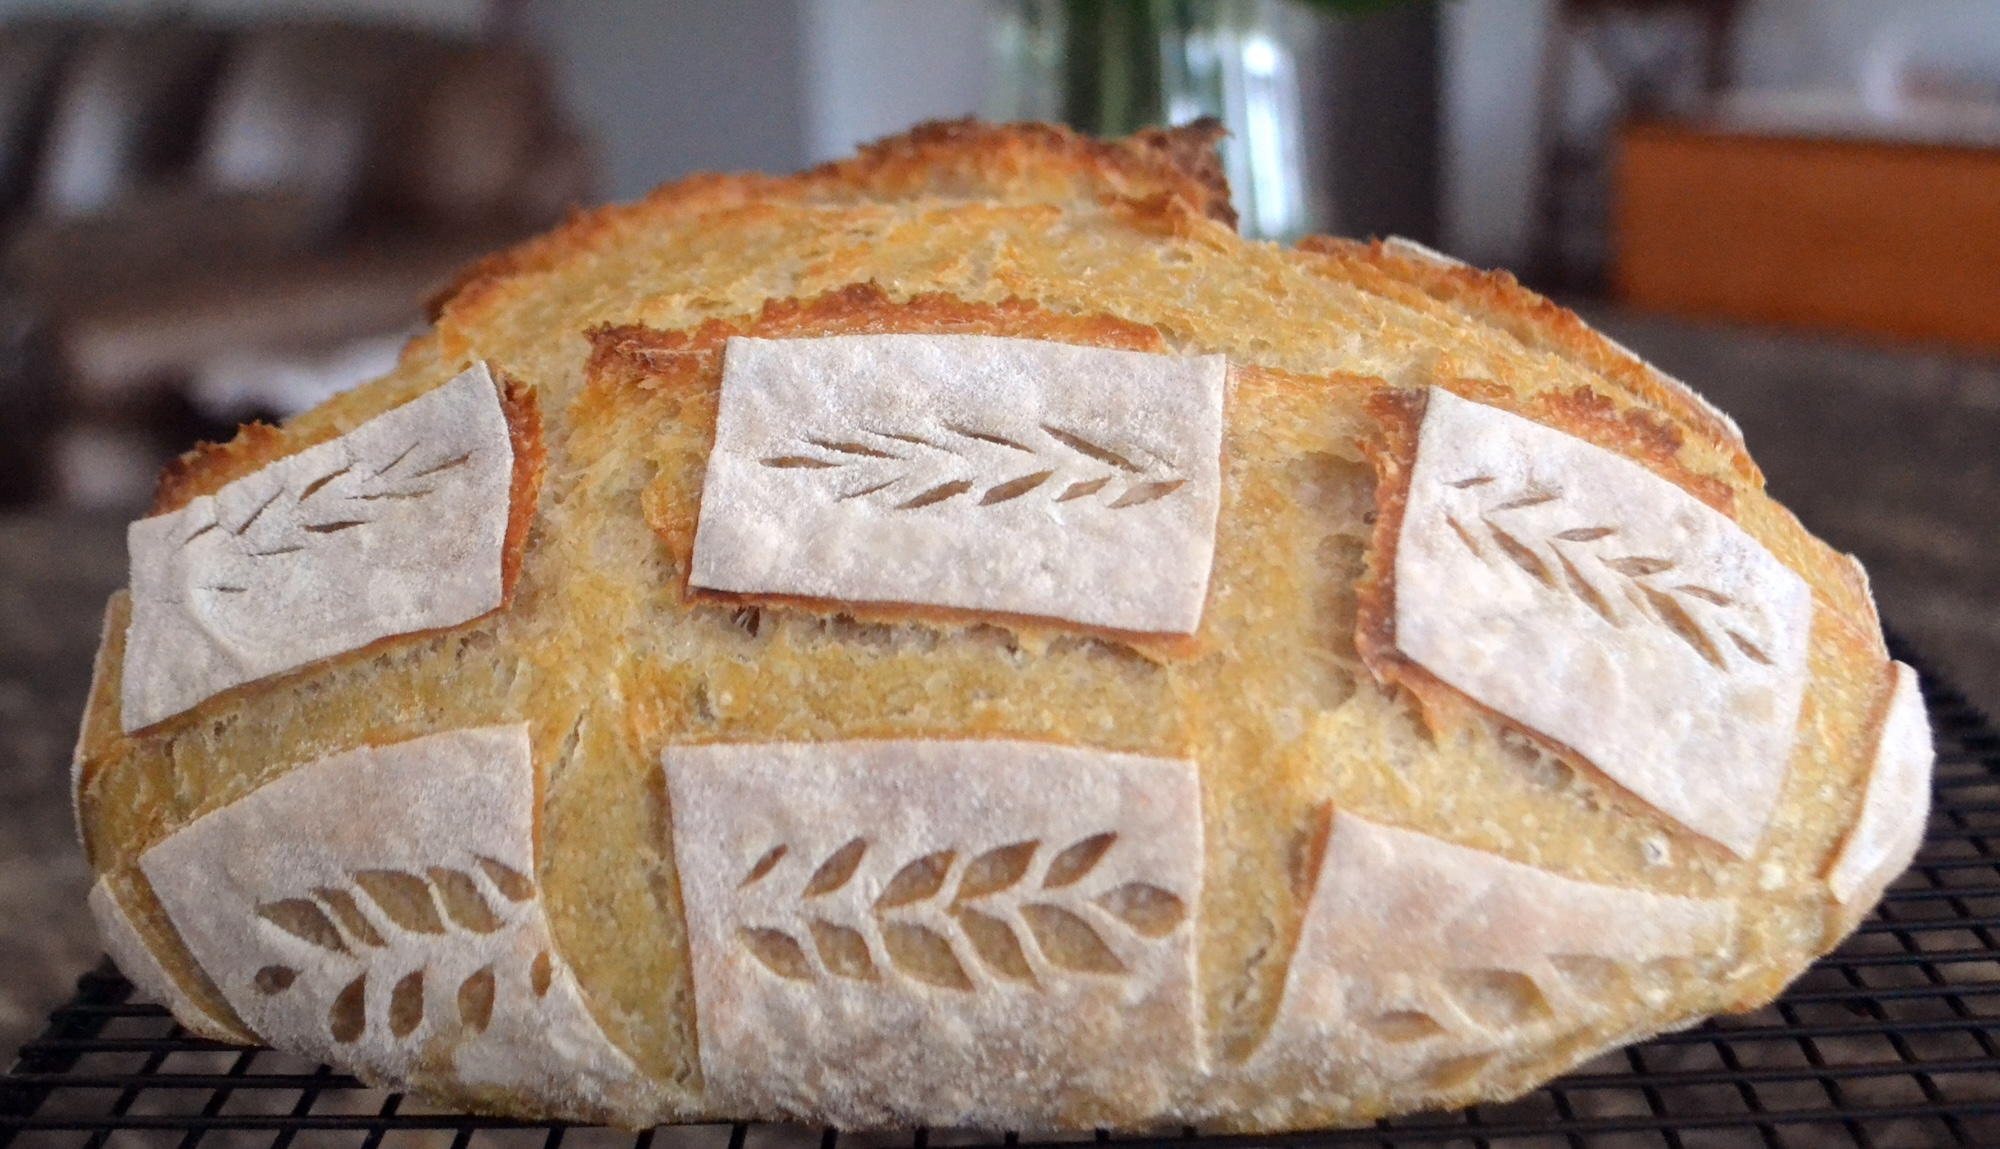
\includegraphics[width=\textwidth]{artistic-scoring}
  \caption[Marquage artistique]{Un pain de Nancy~Anne présentant un motif de
      marquage artistique.  Le contraste élevé a été obtenu en frottant la surface de la pâte
      avec de la farine de riz avant la cuisson. Son compte Instagram
      \texttt{simply.beautiful.sourdough} est spécialisé pour montrer de beaux
      motifs de marquage artistique.}%
  \label{fig:artistic-scoring}
\end{figure}

La coupe de marquage est faite à un angle de \qty{45}{\angle} par rapport à la surface de la pâte, légèrement décalée du centre de la pâte. Avec la coupe à \qty{45}{\angle} angle, le côté superposé montera plus dans le four que l'autre côté.
De cette façon, vous obtiendrez une soi-disant \emph{oreille} sur le pain final.
L'oreille est un bord fin et croustillant qui offre une texture intrigante
lorsqu'on mange. Le bord fin est généralement un peu plus foncé après la cuisson
et offre donc une saveur supplémentaire. À mon avis, l'oreille fait
d'un bon pain, un excellent pain.

\begin{figure}[htb!]
  \includegraphics[width=\textwidth]{bread-scoring-angle}
  \caption[Angle de marquage]{L'angle de \qty{45}{\angle} auquel vous incisez la
      pâte est relatif à la surface de la pâte.  Lorsque vous incisez plus vers
      le côté, vous devez ajuster l'angle pour obtenir l'oreille sur votre
      pain.}%
  \label{fig:scoring-angle}
\end{figure}

L'incision réelle est faite avec un couteau très tranchant, ou mieux, une lame de rasoir.
Vous pouvez utiliser la lame de rasoir directement ou l'attacher à un bâtonnet de bois.
La lame de rasoir offre une meilleure flexibilité que le couteau tranchant.
Quoi qu'il en soit, la lame doit être aussi tranchante que possible. De cette façon, lorsque vous coupez,
la pâte n'est pas déchirée et présente une incision propre, sans bords déchiquetés.
Pour simplifier le scoring, la surface de votre pâte doit être un peu séchée.
De cette façon, il est beaucoup plus facile de faire l'incision.
Pour cette raison, il est crucial de frotter votre pâte avec un peu de farine
avant de la placer dans la banneton. La farine sèche absorbera une partie de l'humidité des couches extérieures de votre pâte. C'est particulièrement important
lorsqu'on travaille avec des pâtes fermentées à température ambiante. Une pâte fermentée au froid est beaucoup plus facile à marquer en raison de la faible viscosité de la pâte. La pâte à température ambiante est beaucoup plus difficile à marquer. L'incision de marquage se déchire beaucoup plus facilement. Avec une incision irrégulière, la pâte a moins de chances de lever correctement dans le four. Il y a des chances que vous n'obteniez pas l'oreille mentionnée précédemment. Pour cette raison, il est particulièrement important de sécher la surface. Le marquage deviendra beaucoup plus facile.

\begin{figure}[htb!]
  \includegraphics[width=\textwidth]{dry-dough-surface}
  \caption[Séchage de la surface de la pâte]{En appliquant de la farine à la surface de votre pâte après le façonnage, la partie externe de la pâte se dessèche un peu. Cela facilite beaucoup le marquage car l'incision est moins susceptible de se déchirer.}%
  \label{fig:dried-out-dough-scoring}
\end{figure}


Le marquage nécessite beaucoup de pratique. Pour cette raison, je recommande
de s'entraîner à faire l'incision après avoir créé la force de la pâte. La pâte
sera très humide et collante. Vous pouvez utiliser un couteau ou une lame de rasoir
pour pratiquer la technique. Attendez quelques minutes puis arrondissez à nouveau
la pâte. Vous pouvez vous entraîner aussi longtemps que vous le souhaitez
jusqu'à ce que vous soyez satisfait de votre technique. Après la fermentation, vous avez seulement une seule chance de pratiquer le marquage. C'est soit réussir, soit rater.

Un truc supplémentaire qui peut vous aider à combiner les bénéfices
de la fermentation à température ambiante et le marquage facile de la fermentation à froid
est de placer votre pâte dans le congélateur pendant 30 minutes avant la cuisson.
Une fois que vous remarquez que votre pâte a presque fini de fermenter, déplacez-la vers le
congélateur. Le congélateur va encore plus sécher la surface et faciliter
le marquage.

Un autre truc intéressant est de cuire votre pâte pendant 30 secondes sans vapeur.
L'air chaud va encore plus sécher la surface de la pâte et simplifier
la technique de marquage. Expérimentez avec le timing pour identifier votre point de mire personnel.